% Options for packages loaded elsewhere
\PassOptionsToPackage{unicode}{hyperref}
\PassOptionsToPackage{hyphens}{url}
%
\documentclass[
]{book}
\usepackage{lmodern}
\usepackage{amssymb,amsmath}
\usepackage{ifxetex,ifluatex}
\ifnum 0\ifxetex 1\fi\ifluatex 1\fi=0 % if pdftex
  \usepackage[T1]{fontenc}
  \usepackage[utf8]{inputenc}
  \usepackage{textcomp} % provide euro and other symbols
\else % if luatex or xetex
  \usepackage{unicode-math}
  \defaultfontfeatures{Scale=MatchLowercase}
  \defaultfontfeatures[\rmfamily]{Ligatures=TeX,Scale=1}
\fi
% Use upquote if available, for straight quotes in verbatim environments
\IfFileExists{upquote.sty}{\usepackage{upquote}}{}
\IfFileExists{microtype.sty}{% use microtype if available
  \usepackage[]{microtype}
  \UseMicrotypeSet[protrusion]{basicmath} % disable protrusion for tt fonts
}{}
\makeatletter
\@ifundefined{KOMAClassName}{% if non-KOMA class
  \IfFileExists{parskip.sty}{%
    \usepackage{parskip}
  }{% else
    \setlength{\parindent}{0pt}
    \setlength{\parskip}{6pt plus 2pt minus 1pt}}
}{% if KOMA class
  \KOMAoptions{parskip=half}}
\makeatother
\usepackage{xcolor}
\IfFileExists{xurl.sty}{\usepackage{xurl}}{} % add URL line breaks if available
\IfFileExists{bookmark.sty}{\usepackage{bookmark}}{\usepackage{hyperref}}
\hypersetup{
  pdftitle={New User Guide for Drones in the UC System},
  pdfauthor={UC Center of Excellence on UAS Safety},
  hidelinks,
  pdfcreator={LaTeX via pandoc}}
\urlstyle{same} % disable monospaced font for URLs
\usepackage{longtable,booktabs}
% Correct order of tables after \paragraph or \subparagraph
\usepackage{etoolbox}
\makeatletter
\patchcmd\longtable{\par}{\if@noskipsec\mbox{}\fi\par}{}{}
\makeatother
% Allow footnotes in longtable head/foot
\IfFileExists{footnotehyper.sty}{\usepackage{footnotehyper}}{\usepackage{footnote}}
\makesavenoteenv{longtable}
\usepackage{graphicx,grffile}
\makeatletter
\def\maxwidth{\ifdim\Gin@nat@width>\linewidth\linewidth\else\Gin@nat@width\fi}
\def\maxheight{\ifdim\Gin@nat@height>\textheight\textheight\else\Gin@nat@height\fi}
\makeatother
% Scale images if necessary, so that they will not overflow the page
% margins by default, and it is still possible to overwrite the defaults
% using explicit options in \includegraphics[width, height, ...]{}
\setkeys{Gin}{width=\maxwidth,height=\maxheight,keepaspectratio}
% Set default figure placement to htbp
\makeatletter
\def\fps@figure{htbp}
\makeatother
\setlength{\emergencystretch}{3em} % prevent overfull lines
\providecommand{\tightlist}{%
  \setlength{\itemsep}{0pt}\setlength{\parskip}{0pt}}
\setcounter{secnumdepth}{5}
\usepackage{booktabs}
\usepackage[margin=1.0in]{geometry}
\usepackage{parskip}
\usepackage{titletoc}
\usepackage[hyphens]{url}
\usepackage{pifont}
\usepackage{amsmath}
\usepackage{amsfonts}
\usepackage{amssymb}
\usepackage[]{natbib}
\bibliographystyle{apalike}

\title{New User Guide for Drones in the UC System}
\author{UC Center of Excellence on UAS Safety}
\date{}

\begin{document}
\maketitle

{
\setcounter{tocdepth}{1}
\tableofcontents
}
\hypertarget{introduction}{%
\chapter*{Introduction}\label{introduction}}
\addcontentsline{toc}{chapter}{Introduction}

\begin{center}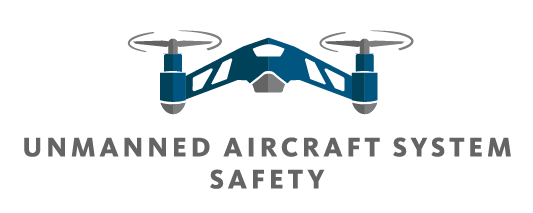
\includegraphics[width=0.5\linewidth]{images/COE_logo} \end{center}

This guide will walk you through the steps for you start flying for your work or research. This page will be a work in progress and new resources will be added periodically. Feel free to reach out to us at \href{mailto:UASSafety@ucmerced.edu}{\nolinkurl{UASSafety@ucmerced.edu}} if you have any questions or would like to see additional resources added.

\hypertarget{uc-drone-policy}{%
\section*{UC Drone Policy}\label{uc-drone-policy}}
\addcontentsline{toc}{section}{UC Drone Policy}

There is a University of California Drone Policy that governs the use of drones owned by the University of California, the use of drones at any University property, or the use of drones for any University purpose (including teaching, outreach and research). More information about the UC UAS Policy can be found in the UC UAS Policy Guidance Document located at \url{http://UCDrones.github.io/Policy_Guidance/}

\hypertarget{policy-requirements}{%
\subsection*{Policy Requirements}\label{policy-requirements}}
\addcontentsline{toc}{subsection}{Policy Requirements}

The Policy establishes that anyone who seeks to operate a UAS under the jurisdiction of the policy must:

\begin{itemize}
\tightlist
\item
  Comply with any applicable regulation, including but not limited to any applicable FAA regulation.
\item
  Have prior approval from the Campus Drone Person or the Systemwide Designated Authority.
\item
  Operate in a manner that ensures public safety, right to privacy, civil rights and civil liberties.
\item
  Maintain sufficient liability insurance coverage.
\end{itemize}

The UC Center of Excellence on UAS Safety is here to help you guide you through the process.

\hypertarget{step-by-step-uc-drone-process}{%
\subsection*{Step-by-step UC Drone Process}\label{step-by-step-uc-drone-process}}
\addcontentsline{toc}{subsection}{Step-by-step UC Drone Process}

\begin{enumerate}
\def\labelenumi{\arabic{enumi}.}
\tightlist
\item
  Register your drone with the \protect\hyperlink{ch-register}{FAA} and UC
\item
  Get an \protect\hyperlink{ch-get-license}{FAA Drone License} (or figure out if you're \protect\hyperlink{ch-license}{exempt}) and register yourself with the UC
\item
  Find a place to fly - review \protect\hyperlink{ch-airspace-info}{airspace}, \protect\hyperlink{ch-safety-guidelines}{safety guidelines} and \protect\hyperlink{ch-local-UAS-regulations}{local regulations}
\item
  Submit a UC Flight Request
\item
  Fly Safely
\item
  Submit a Post-Flight Report
\end{enumerate}

\hypertarget{outline}{%
\section*{Outline}\label{outline}}
\addcontentsline{toc}{section}{Outline}

\hypertarget{complying-with-regulations}{%
\subsection*{Complying with Regulations}\label{complying-with-regulations}}
\addcontentsline{toc}{subsection}{Complying with Regulations}

\begin{itemize}
\tightlist
\item
  \protect\hyperlink{ch-register}{Register your Drone with the FAA}
\item
  \protect\hyperlink{ch-license}{Do I need a License?}
\item
  \protect\hyperlink{ch-get-license}{How to get a License}
\item
  \protect\hyperlink{ch-airspace-info}{How to get Airspace Information}
\end{itemize}

\hypertarget{getting-uc-approval}{%
\subsection*{Getting UC Approval}\label{getting-uc-approval}}
\addcontentsline{toc}{subsection}{Getting UC Approval}

\begin{itemize}
\tightlist
\item
  \protect\hyperlink{ch-about-UCdrones}{About UC Drones}
\item
  Registering your drone with your campus
\item
  Creating a flight request
\item
  Post-Flight Reporting
\item
  Where to get more help
\end{itemize}

\hypertarget{planning-for-safety}{%
\subsection*{Planning for Safety}\label{planning-for-safety}}
\addcontentsline{toc}{subsection}{Planning for Safety}

\begin{itemize}
\tightlist
\item
  \protect\hyperlink{ch-safety-guidelines}{Safety Guidelines}
\item
  Field Safety
\item
  Fire Safety
\item
  Working around people and non-participants
\item
  Writing a Privacy Plan
\item
  \protect\hyperlink{ch-fire-safety}{Fire Safety}
\end{itemize}

\hypertarget{insurance}{%
\subsection*{Insurance}\label{insurance}}
\addcontentsline{toc}{subsection}{Insurance}

\begin{itemize}
\tightlist
\item
  \protect\hyperlink{ch-liability-insurance}{UAS Liability Insurance}
\item
  \protect\hyperlink{ch-hull-insurance}{UAS Property Insurance}
\end{itemize}

\hypertarget{more-details}{%
\subsection*{More Details}\label{more-details}}
\addcontentsline{toc}{subsection}{More Details}

\begin{itemize}
\tightlist
\item
  \protect\hyperlink{ch-common-UAS-violations}{Common UAS Violations}
\item
  \protect\hyperlink{ch-uas-accident}{Reporting UAS accidents}
\item
  \protect\hyperlink{ch-local-UAS-regulations}{Local UAS Regulations}
\item
  \protect\hyperlink{ch-replace-license}{How do I update or replace my License?}
\end{itemize}

\hypertarget{part-getting-started}{%
\part{Getting Started}\label{part-getting-started}}

\hypertarget{ch-register}{%
\chapter{Register your Drone}\label{ch-register}}

\begin{quote}
This page is for the registration of your drone with the Federal Aviation Administration. For information on how to register your drone with the UC system, see Chapter.
\end{quote}

All drones that weigh more than 0.55 lbs (250 grams) must be registered with the Federal Aviation Administration (FAA) to it's legal owner.

Any drone purchased through the University of California for university business, including teaching and research, is owned by the Regents of the University of California.

You can register the drone through the FAA Drone Zone (\url{https://faadronezone.faa.gov}). Registration costs only \$5 per aircraft and only takes a couple of minutes.

\hypertarget{create-an-account-at-dronezone}{%
\section{Create an account at DroneZone}\label{create-an-account-at-dronezone}}

Head to the FAA DroneZone (\url{https://faadronezone.faa.gov}) and select ``I fly under Part 107 or as a Public Aircraft'' \ref{fig:reg-page}

\begin{figure}

{\centering 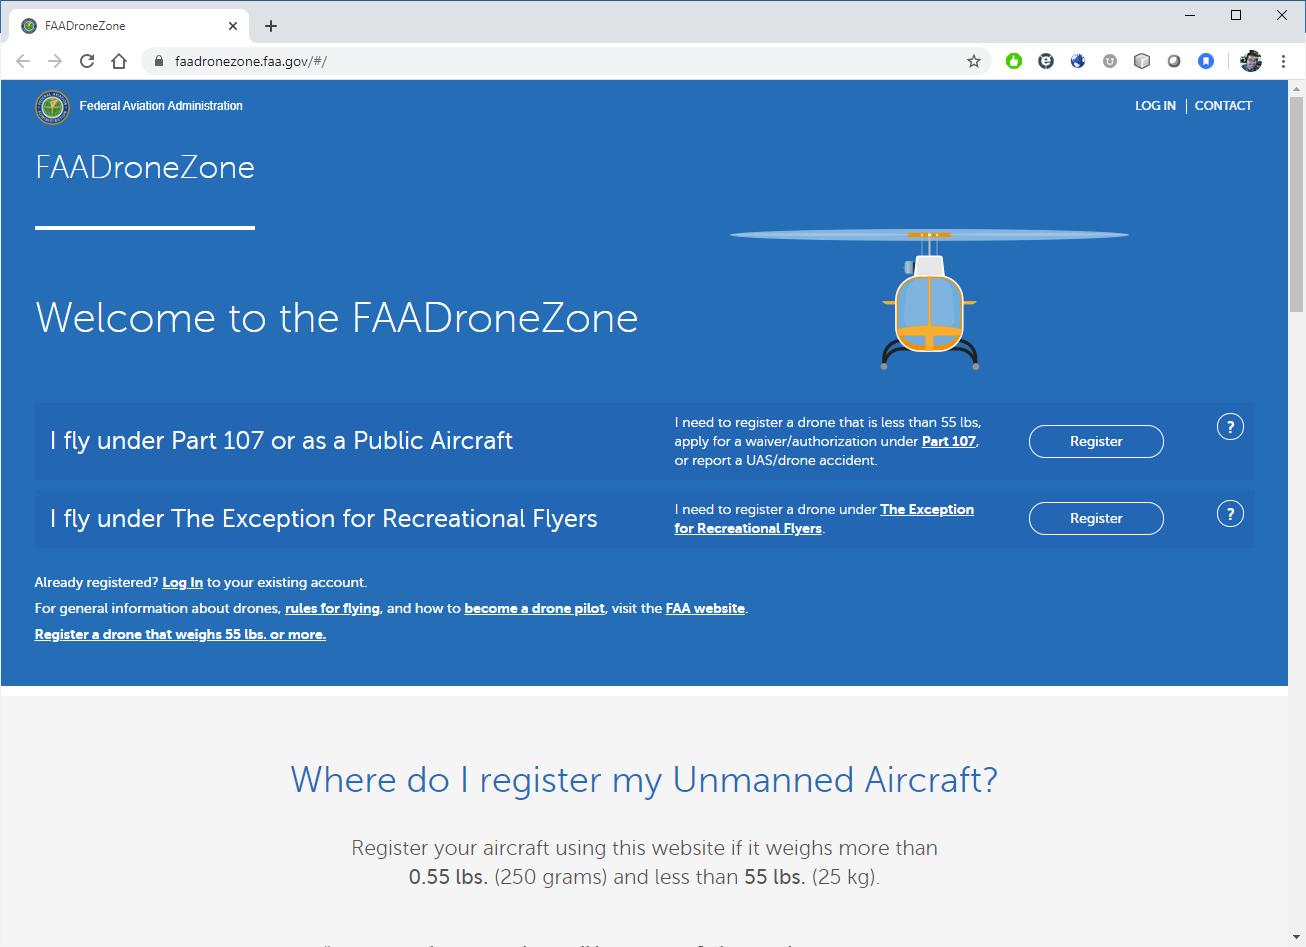
\includegraphics[width=0.8\linewidth]{images/reg_site} 

}

\caption{FAA DroneZone}\label{fig:reg-page}
\end{figure}

\begin{quote}
Unfortunately, the FAA's drone registration website does not allow you to register drones for multiple groups or organizations. If you're registering a drone on behalf of the University of California, you should use your UC email address as your account log in, and use a personal email address account for any personally-owned drones.
\end{quote}

When you enter your Part 107 Account information, enter \textbf{Regents of the University of California} as your Part 107 Account Name to correctly register the drone to the UC system.

\hypertarget{drone-registration}{%
\section{Drone Registration}\label{drone-registration}}

Once you have an account, on the dashboard will be an option to `Manage sUAS Inventory.' On that page, you'll be able to `Add UAS' (in the upper right corner). This will bring up a dialog box (Figure \ref{fig:add-UAS}) for you to enter your information. Enter all the relevant information.

\begin{figure}

{\centering 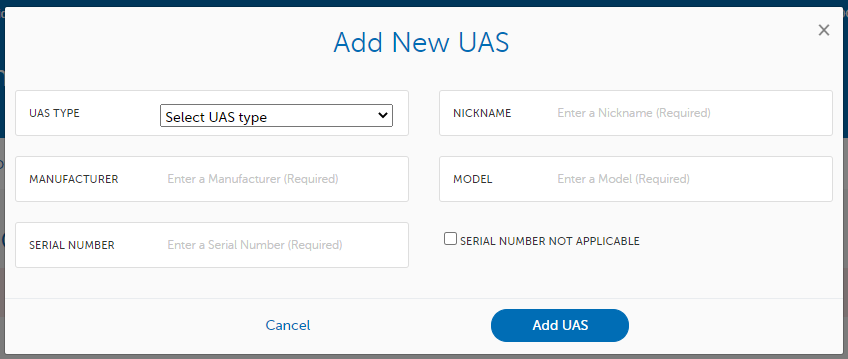
\includegraphics[width=0.8\linewidth]{images/Add_new_UAS} 

}

\caption{Add new UAS Dialog Box}\label{fig:add-UAS}
\end{figure}

Once completed, `Your Shopping Cart' will now show this drone's information and a new buttom for `Checkout' will appear. Click the button and the system will guide you through paying for the registration fee.

\hypertarget{registration-certificate}{%
\section{Registration Certificate}\label{registration-certificate}}

Upon completion of paying for registration, the DroneZone will send you two emails, one with a receipt of payment and the other is a pdf copy of your UAS registration certificate (Figure \ref{fig:reg-cert}). Keep a copy of this registration certificate available at all times while you operate. This can be done by either printing it out and placing it with your drone, or keeping a digital copy on your phone.

\begin{figure}

{\centering 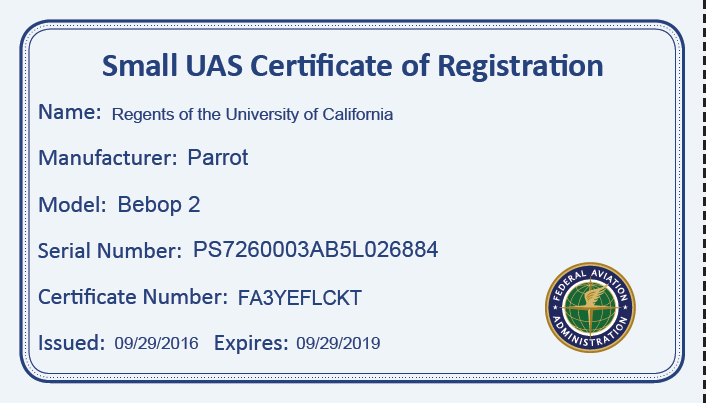
\includegraphics[width=0.5\linewidth]{images/reg_cert} 

}

\caption{Example UAS Registration Certificate}\label{fig:reg-cert}
\end{figure}

\hypertarget{marking-the-drone}{%
\section{Marking the Drone}\label{marking-the-drone}}

Your drone's registration number is the 10 digit alphanumeric code that starts with \textbf{FA}. You must mark this on your drone on an external location, where it can be plainly visible.

We recommend either using a permanent oil-based fine tip paint marker (Figure \ref{fig:markers}) or creating a label that can be strongly affixed to the drone. We've found that regular sharpies or markers are rubbed off too easily to be effective.

\begin{figure}

{\centering 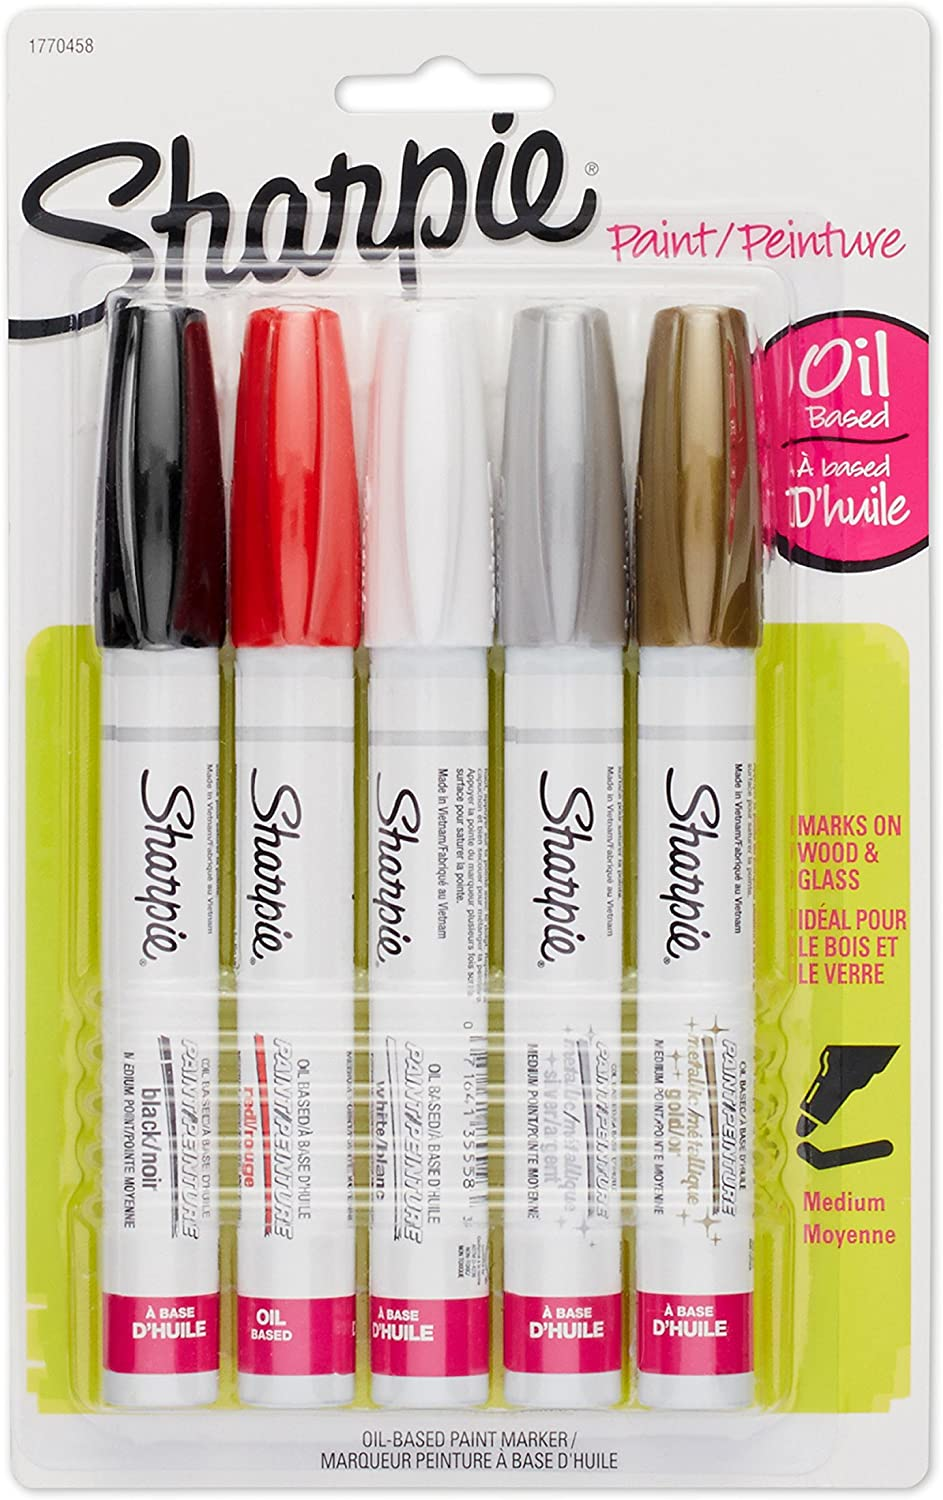
\includegraphics[width=0.5\linewidth]{images/oil-based-markers} 

}

\caption{Oil-Based Paint Markers}\label{fig:markers}
\end{figure}

If you'll be working with a fleet of aircraft, it may also be useful to mark the `nickname' of the drone as well.

\hypertarget{ch-license}{%
\chapter{Do I need an FAA License?}\label{ch-license}}

When operating a drone within the US, there are two different options for regulations: Part 107 Small UAS regulations or the Exception for Limited Recreational Use. By default, UAS operations fall under Part 107 Small UAS regulations, unless you can meet the requirements for the exception for Recreational Use. Part 107 requires that all pilots have a Remote Pilot Certificate with an sUAS rating, more commonly known as a `Drone License,' whereas Recreational Use does not require a Drone License.

Many researchers opt to get a Drone License for their research needs, but a Drone License does cost \$150 and will take some time to study and prepare for. With the updates introduced in the FAA Reauthorization Act of 2018 (P.L. 115-254), there are more exceptions available in which you may not need to obtain the license.

\begin{quote}
This page is for the Federal Aviation Administration licensing requirements for UAS use. UC Policy will still require a flight request and post flight reporting, regardless of FAA licensing requirements. More information on the UC policy can be found in Chapter .
\end{quote}

\hypertarget{what-is-the-difference}{%
\section{What is the difference?}\label{what-is-the-difference}}

Under Part 107

\begin{itemize}
\tightlist
\item
  Drone License required
\item
  Any purpose
\item
  `Fly only when it is safe'
\item
  May request special permissions

  \begin{itemize}
  \tightlist
  \item
    Above FAA Facility Map altitudes
  \item
    Over People, BVLOS, More than 1 drone at a time
  \end{itemize}
\end{itemize}

Under Recreational Exception

\begin{itemize}
\tightlist
\item
  No license required
\item
  Recreation or Approved Academic Activities
\item
  `Fly only in safe locations'
\item
  No allowances for advanced operations
\end{itemize}

\hypertarget{when-are-you-exempt-from-a-drone-license}{%
\section{When are you Exempt from a drone license}\label{when-are-you-exempt-from-a-drone-license}}

You may not need a drone license if your flight operations can fit under the stipulations listed for `recreational' activities \textbf{and} your flight operations are related to

\begin{itemize}
\tightlist
\item
  Coursework
\item
  Instruction of students
\item
  Academic or research related uses of unmanned aircraft systems that have been approved by the institution
\item
  Activities undertaken by the institution as part of research projects
\item
  Other academic activities approved by the institution
\end{itemize}

\hypertarget{what-are-the-stipulations-for-recreational-and-approved-academic-activities}{%
\section{What are the stipulations for `Recreational' and approved `Academic' activities?}\label{what-are-the-stipulations-for-recreational-and-approved-academic-activities}}

Recreational flight operations, despite what you see on YouTube, have strict requirements:

\begin{itemize}
\tightlist
\item
  Only fly below 400 ft
\item
  Must stay within Visual Line of Sight
\item
  Must fly only in safe areas and no closer than 25 ft to any individuals
\item
  Must use an established safety line to separate all operations from spectators and bystanders
\item
  Must get FAA authorization to fly in Controlled Airspace (Class B, Class C, Class D and surface Class E)
\item
  Never fly over any person or moving vehicle
\item
  Never interfere with any manned aircraft or emergency response activity
\item
  Never fly under the influence of drugs or alcohol
\item
  Never operate in a careless or reckless manner
\end{itemize}

This is in addition to existing UAS operating restrictions under 14 CFR 107:

\begin{itemize}
\tightlist
\item
  No operating from a moving vehicle
\item
  No operating more than one vehicle at a time
\item
  No operating faster than 100 mph
\item
  No operating when the weather visibility is less than 3 miles
\item
  No operating closer than 500 ft below a cloud, or within 2000 ft horizontally from a cloud or fog layer
\end{itemize}

\hypertarget{other-situations}{%
\section{Other Situations}\label{other-situations}}

There are other conditions that may require a closer evaluation, including whether you're a US citizen or if you plan on flying internationally. If you have any questions, feel free to reach out to \href{mailto:UASsafety@ucmerced.edu}{\nolinkurl{UASsafety@ucmerced.edu}} for a consultation.

Other scenarios that may require a closer look

\begin{itemize}
\tightlist
\item
  Performing a demonstration
\item
  Not a US citizen
\item
  Flying above 400 ft AGL
\item
  Flying in fog or with limited visibility
\item
  Flying at night
\item
  Flying internationally
\end{itemize}

\hypertarget{frequently-asked-questions}{%
\section{Frequently Asked Questions}\label{frequently-asked-questions}}

\textbf{When doing an academic activity, which set of regulations is better?}

There are advantages and disadvantages to both scenarios. In many cases, the new `Recreational Operations' may be the fastest path forward for simple, rural flight operations. At the current time, academic UAS activities that plan on flying in certain controlled airspace areas, over occupied structures, within 25 ft of another person, or outside of a reasonably controlled flying site, should proceed with 14 CFR 107 regulations.

\textbf{What does it mean to get approval from the FAA to operate within controlled airspace?}

The FAA is mandating that all controlled airspace access requests for recreational operations be routed through the Low Altitude Authorization Notification Capability system (LAANC) and not by calling the local airport tower. The LAANC system can provide instantaneous authorization via a 3rd party application such as Airmap, KittyHawk, or UASideKick for flight requests below a certain altitude depending on your location.

\textbf{I am planning to fly over a research site that is access controlled and the airspace is uncontrolled, do I need a Drone License?}

Typically not. This common scenario will typically meet the necessary site requirements for Recreational Operations.

\textbf{I am planning to fly along the beach to monitor coastal erosion, do I need a Drone License?}

Unless the beach is to be closed to the public, this scenario will likely require a Drone License.

\textbf{I am planning on flying in the campus quad to test a flight controller, do I need a Drone License?}

If the airspace is uncontrolled (Class G), and the area within the campus quad is sufficiently cleared and closed to non-participants, then you do not need a Drone License. If you want to fly on campus at UCI, UCLA or UCSB, then you will need to obtain an Airspace Authorization via LAANC.

\textbf{I do not have a Drone License, can I do a coursework assignment on the use of drones in building inspections?}

You may be able to do some flying without a drone license, however, you will not be allowed to fly over a building and must stay at least 25 ft from all non-participants, which may limit your ability to conduct effective analysis.

\textbf{I am a graduate student Teaching Assistant and I would like to teach my students how to fly a drone? Do I need a license? Do the students need a license?}

If the site is sufficiently cleared and closed to non-participants, than everyone may have a chance to learn how to fly a drone without a drone license and any instructor will also not need to have a license. However, additional safety precautions may be necessary and as an instructor, you will be responsible for ensuring the safety of the students and the site.

\hypertarget{ch-get-license}{%
\chapter{How to get a License}\label{ch-get-license}}

Obtaining a Remote Pilot Certificate, or more commmonly known as a drone license, is relatively straight-forward

\hypertarget{drone-license-exam}{%
\section{Drone License Exam}\label{drone-license-exam}}

The drone license exam (airman knowledge test) is a 120 minute, 60 question exam that goes over a wide range of topics. The topics covered on the exam can be broken down into 12 sections as follows:

\begin{enumerate}
\def\labelenumi{\arabic{enumi}.}
\tightlist
\item
  General UAS regulations
\item
  Airspace classifications
\item
  Aviation weather sources
\item
  Loading and Performance
\item
  Emergency procedures
\item
  Crew resource management
\item
  Radio communication procedures
\item
  Determining UAS performance
\item
  Physiological effects of drugs and alcohol
\item
  Aeronautical decision-making and judgment
\item
  Airport operations
  and
\item
  Maintenance and pre-flight inspection procedures.
\end{enumerate}

A more in depth look at these topics can be found on the FAA's website here: (\url{https://www.faa.gov/regulations_policies/handbooks_manuals/aviation/media/remote_pilot_study_guide.pdf})

Although there are third party ``Ground school'' courses offered for a fee we have found freely available resources to be just as effective.

\hypertarget{free-study-resources}{%
\section{Free study resources}\label{free-study-resources}}

Here are a few free study resources to aid in studying for the exam:

\begin{itemize}
\tightlist
\item
  (\url{https://jrupprechtlaw.com/part-107-test-study-guide})
\item
  (\url{https://northrup.photo/free-faa-part-107-suas-drone-certification-study-guide/})
\item
  (\url{https://www.3dr.com/docs/faa-part-107-study-guide/part-107-certification-official-study-resources/})
\end{itemize}

\hypertarget{drone-license-eligibility}{%
\section{Drone License Eligibility}\label{drone-license-eligibility}}

In order to be eligible to obtain a Remote Pilot Certificate, you must meet the following requirements:

\begin{itemize}
\tightlist
\item
  Be at least 16 years of age
\item
  Be able to read, speak and understand the English language. If the applicant is unable to meet one of these requirements due to medical reasons, the FAA may place such operation limitations on that applicant's certificate as are necessary for the safe operation of the small unmanned aircraft.
\item
  Not know or have reason to know that he or she has a physical or mental condition that would interfere with the safe operation of a small unmanned aircraft system.
\end{itemize}

However, to take the FAA Airman Knowledge Exam, the proponent must prove their identity with a valid photo ID that includes their date of birth, signature and physical, residential address.

For U.S. Citizens and U.S. Resident Aliens, this may be accomplished with one of the following:

\begin{itemize}
\tightlist
\item
  Driver Permit or License issued by a U.S. state or territory
\item
  U.S. Government Identification Card
\item
  U.S. Military Identification Card
\item
  Passport
\item
  Alien Residency Card
\end{itemize}

For Non-U.S. Citizens, this may be accomplished with one of the following:

\begin{itemize}
\tightlist
\item
  Passport and a Driver permit or license issued by a U.S. state or territory.
\item
  Passport and an Identification card issued by any governmental entity.
\end{itemize}

\hypertarget{ch-airspace-info}{%
\chapter{How to get Airspace information}\label{ch-airspace-info}}

When your figuring out where you want to fly, you're typically thinking about your research objectives on the ground. But you must also think about whether or not it will be safe to fly a drone in the airspace at that location. You won't find this information on Google Maps though - you need to check the Airspace Maps or Aviation Charts.

Reading an Airspace Map is not like reading Google Maps - you'll rarely see roads or buildings marked - instead you'll be presented with a whole new set of symbols and strange codes. But they're all very important to convey a dense set of aviation information. Luckily with drones, you won't have to worry about most of it, but there's still some very important pieces of information you need to know.

\begin{quote}
There's a lot of rules about flying drones and many of them are related to where and how risky. For more information about Airspace Class and their rules, check out the UAS Regulations and the Learning about Airspace pages.
\end{quote}

\textbf{Things you should look for when reviewing Airspace Information}

\begin{itemize}
\tightlist
\item
  Airspace Class
\item
  Nearby Airports, including smaller ones and helipads
\item
  Potential air traffic patterns
\item
  Special Use Airspace - Military Operating Areas, Controlled Firing Ranges, National Security Areas, and Restricted Areas
\item
  Flying altitude limits within certain zones or grids
\item
  Temporary Flight Restrictions or special alerts
\end{itemize}

So where can you find this information? We recommend two sources:

\begin{itemize}
\tightlist
\item
  Airmap (3rd party application and website)
\item
  Official FAA Sources - VFR Sectional Charts, FAA Facility Maps, TFR/NOTAMs
\end{itemize}

\hypertarget{airmap}{%
\section{Airmap}\label{airmap}}

The most comprehensive and easy to use Drone airspace map system is \href{https://app.airmap.com/}{Airmap}. Just type in your address or find your spot on the map, and see whats around you. Airmap is available as both a webpage (Figure \ref{fig:airmap-web}) and as an app for \href{https://apps.apple.com/us/app/airmap-for-drones/id1042824733}{iOS} or \href{https://play.google.com/store/apps/details?id=com.airmap.airmap\&hl=en_US}{Android} (Figure \ref{fig:airmap}).

Once you find your flying spot on the map, you can evaluate many of the airspace issues you need to look for. For example, in Figure \ref{fig:airmap-web}, the selected flying spot is within a grid box within the purple shaded region.
The text box to the bottom left gives a brief explanation - the purple shaded region is MERCED CLASS E2 airspace - meaning that the location is located within the vicinity of the Merced Airport. Any drone flying within any purple of blue shaded region will require permission from the FAA. Class E2 is the least riskiest of the airport managed airspace (also known as controlled airspace), but still will have some airspace risk with occasional planes and helicopters flying above.

\begin{figure}

{\centering 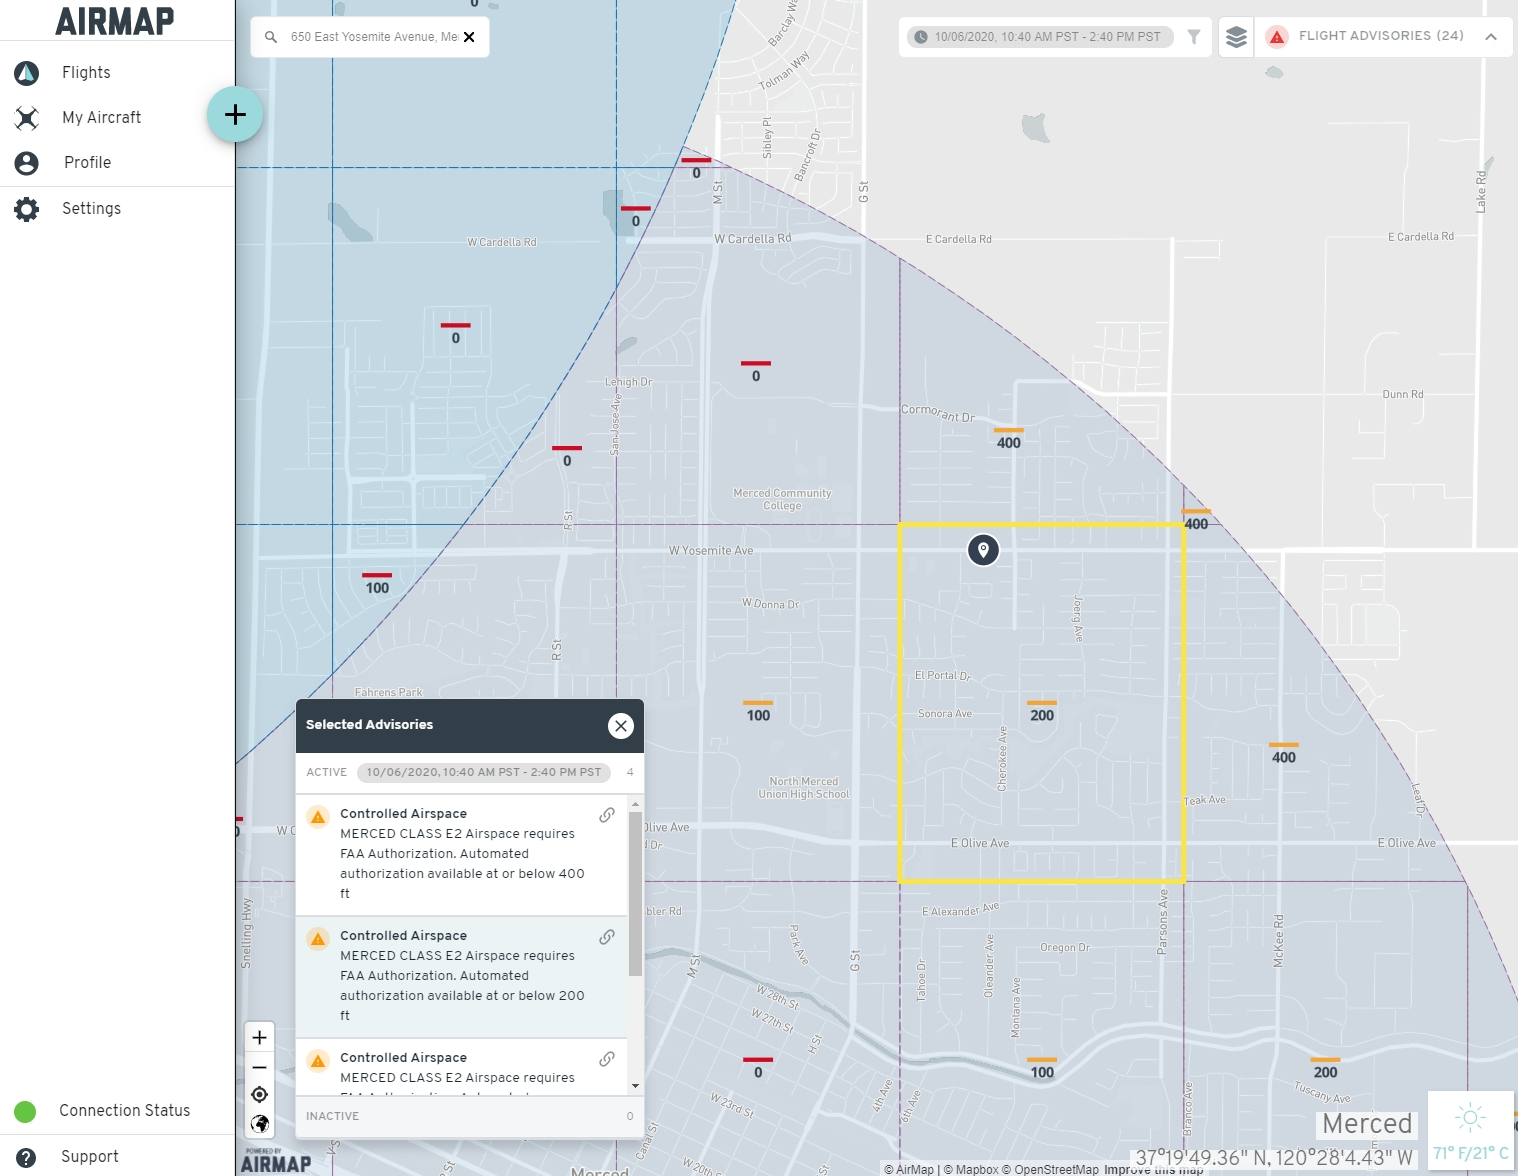
\includegraphics[width=0.85\linewidth]{images/Airmap-webpage} 

}

\caption{Android Airmap Application}\label{fig:airmap-web}
\end{figure}

For requesting permission to fly within a shaded region (controlled airspace), the FAA and the airports have drawn up grids within the shaded regions and labeled each one with a generally safe upper limit for flying. Within the highlighted grid in Figure \ref{fig:airmap-web}, this limit is 200 ft. If you ask the FAA for permission to fly up to 200 ft, you will always be given approval. In general, the farther away you are from the runway, the higher the altitude you will be allowed to fly. But that's not always the case - you'll notice, there are a couple of grids that are marked with a 0 - and yes, that means that the generally safe flying altitude is 0 ft.

\begin{quote}
Need to get FAA permission to fly in one of these areas, head over \protect\hyperlink{ch-LAANC}{here}
\end{quote}

What if you need to fly higher than the altitude listed? If you have a drone pilot license, you may ask the FAA for permission - but it is not guaranteed to be approved. Obtaining permission for flights above the listed altitude can be tricky, so we recommend reaching out to us at \href{mailto:UASsafety@ucmerced.edu}{\nolinkurl{UASsafety@ucmerced.edu}} and we'll be happy to walk you through the process. Reach out to us early - the FAA can take 5-10 days to grant approval so you want to start this process early.

Airmap also does a good job of depicting other airspace issues, such as Special Use Airspace and National Security Areas - marked in red as in Figure \ref{fig:airmap}. Selecting the AIRMAP Recommended Guidelines layer will also show all the helipads and minor airports that are not normally shown on an airspace map. This can be critically important - low flying helicopters and cropdusters that fly out of these unmarked airports are among the most pressing airspace concerns.

\begin{quote}
Make sure you click on the `Layers' Icon next to the Flight Advisories - this allows you to turn on/off different information. For most operations, we recommend selecting the following sets of information:

\begin{itemize}
\tightlist
\item
  FAA Part 107 Certified
\item
  AIRMAP Recommend Guidelines
\item
  Restricted and Special Use Airspace
\item
  National Parks Public Use Limits
\item
  NOAA Regulated Overflight Zones
\item
  Fish and Wildlife Service Lands Use Limits
\item
  Wilderness Areas Use Limits
\end{itemize}
\end{quote}

\begin{figure}

{\centering 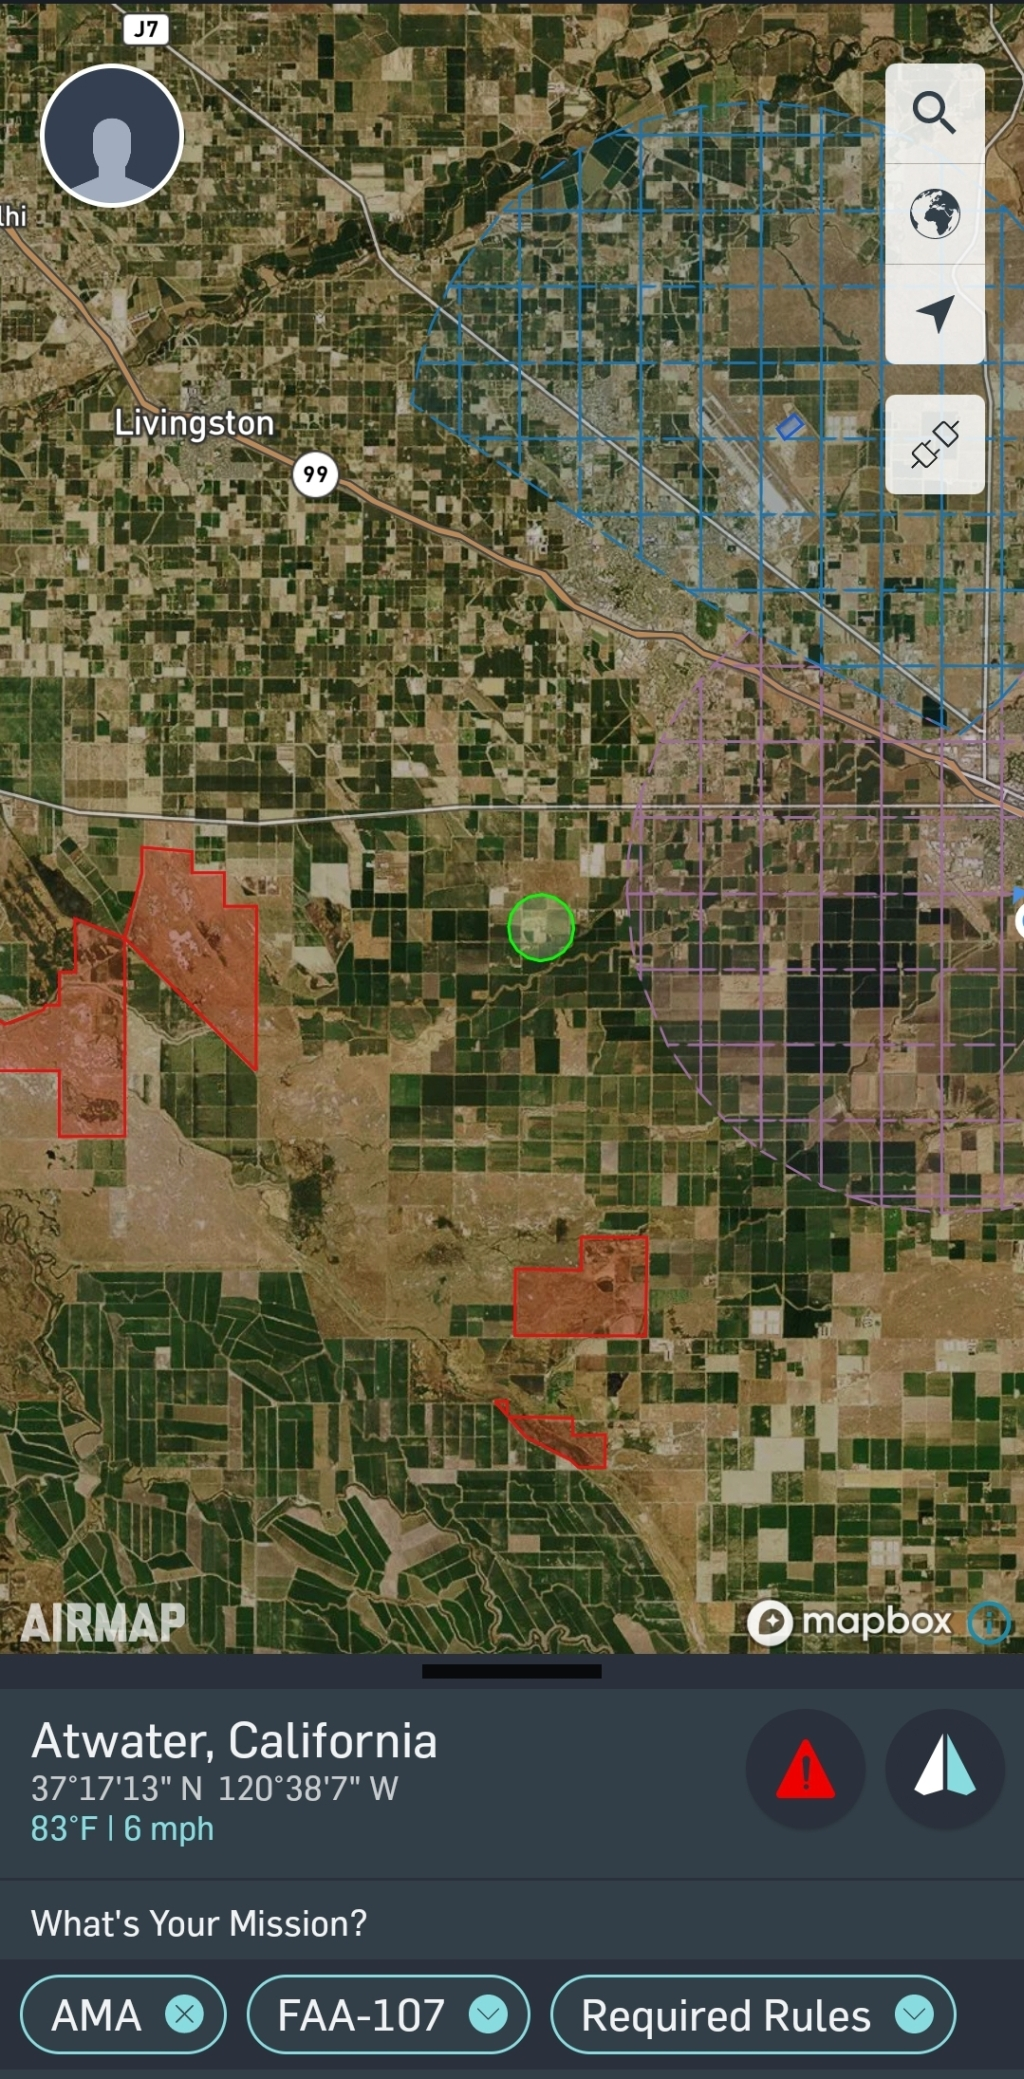
\includegraphics[width=0.5\linewidth]{images/Airmap-Android} 

}

\caption{Android Airmap Application}\label{fig:airmap}
\end{figure}

\hypertarget{the-importance-of-up-to-date-airspace-information}{%
\subsection{The importance of up-to-date Airspace Information}\label{the-importance-of-up-to-date-airspace-information}}

Having the most up-to-date airspace information on hand can make all the difference between having a safe flight and a risky one. One of the advantages of Airmap is that it will also display a number of Temporary Flight Restrictions and Notices to Airman. Especially in California, there are a number of these that we should always keep an eye on:

\begin{itemize}
\tightlist
\item
  \textbf{Disneyland} - Due to National Security Risks, the FAA has banned all aircraft from flying under 3000 ft within 3 miles of Disneyland. This essentially also bans all drones in the area as well.\\
\item
  \textbf{Major League Baseball}, \textbf{National Football League} and \textbf{Division 1 College Football} Regular and Post-Season Games - Similarly to the Disneyland restriction, the FAA has banned all aircraft from flying under 3000 ft within 3 miles of any these games. The ban starts at 1 hour before the games begin to 1 hour after the game ends.\\
\item
  \textbf{Wildfire and other Natural Disasters} - Whenever there is a major catastrophe, keep an eye out for Temporary Flight Restrictions. These will often be very large and prolonged to allow emergency services (firefighting aircraft, medical support, etc) to have priority in these areas. Never fly your drone in a manner that could interfere with emergency services - it is both a Federal offense and a State offense.\\
\item
  \textbf{US President and Vice-President Travel} - The President (30 mile) and Vice-President (5 mile) travel with their own FAA flight restriction zones, similarly prohibiting all aircraft from flying under 3000 ft within their zones.
\end{itemize}

\begin{quote}
As with most drone related rules and regulations, there are nuances and exceptions to TFRs and NOTAMs. If you have a pressing need to operate within a TFR, reach out to us at \href{mailto:UASsafety@ucmerced.edu}{\nolinkurl{UASsafety@ucmerced.edu}} to discuss.
\end{quote}

\hypertarget{official-faa-sources}{%
\section{Official FAA Sources}\label{official-faa-sources}}

Using Airmap is one of the easiest methods for looking up most of the airspace issues. However, it's not always the most detailed nor is it the official source of information. The official sources of information is spread across a handful of different sites:

\begin{itemize}
\tightlist
\item
  Official source of airspace information - \href{https://www.faa.gov/air_traffic/flight_info/aeronav/digital_products/vfr/}{FAA Sectional Charts}
\item
  Official source of altitude grid information - \href{https://faa.maps.arcgis.com/apps/webappviewer/index.html?id=9c2e4406710048e19806ebf6a06754ad}{UAS Facility Maps}
\item
  Official source of TFR or NOTAMS - \href{https://notams.aim.faa.gov/notamSearch/nsapp.html\#/}{FNS NOTAM Search}
\end{itemize}

\begin{quote}
Always check multiple sources - you never know when one source omits an important piece of information. For example, Figure \ref{fig:facility-map} is the default view of Orange County of the UAS Facility Maps, but its doesn't depict one very critical flight restriction.
\end{quote}

\hypertarget{faa-sectional-charts}{%
\subsection{FAA Sectional Charts}\label{faa-sectional-charts}}

\begin{figure}
\centering
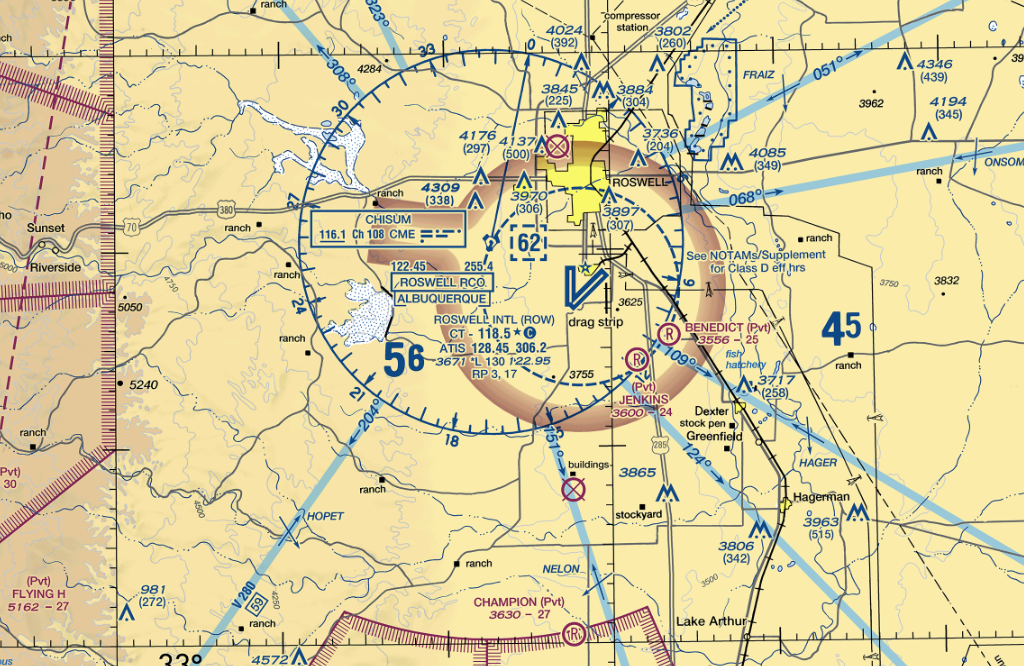
\includegraphics{images/FAA-VFR.png}
\caption{FAA sectional chart}
\end{figure}

Getting information on a specific area's airspace classification has never been easier. The FAA has region specific sectional charts located \href{https://www.faa.gov/air_traffic/flight_info/aeronav/digital_products/vfr/}{here}.

\hypertarget{uas-facility-maps}{%
\subsection{UAS Facility Maps}\label{uas-facility-maps}}

\begin{figure}

{\centering 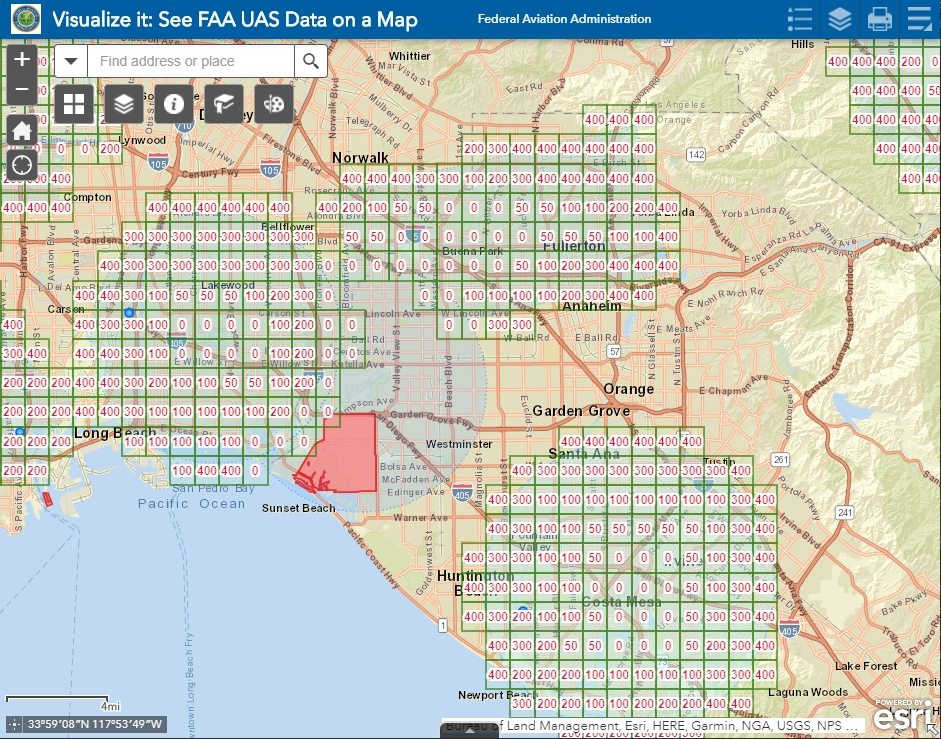
\includegraphics[width=0.9\linewidth]{images/facility-map} 

}

\caption{UAS Facility Map}\label{fig:facility-map}
\end{figure}

UAS Facility Maps show the maximum altitudes around airports where the FAA may authorize drone operations without additional safety analysis. Grids marked in Green are LAANC (Low Altitude Authorization and Notification Capability) enabled - More on that in \protect\hyperlink{ch-LAANC}{LAANC Authorization}.

\hypertarget{notam-or-notice-to-airman}{%
\subsection{NOTAM or Notice To Airman}\label{notam-or-notice-to-airman}}

\begin{figure}
\centering
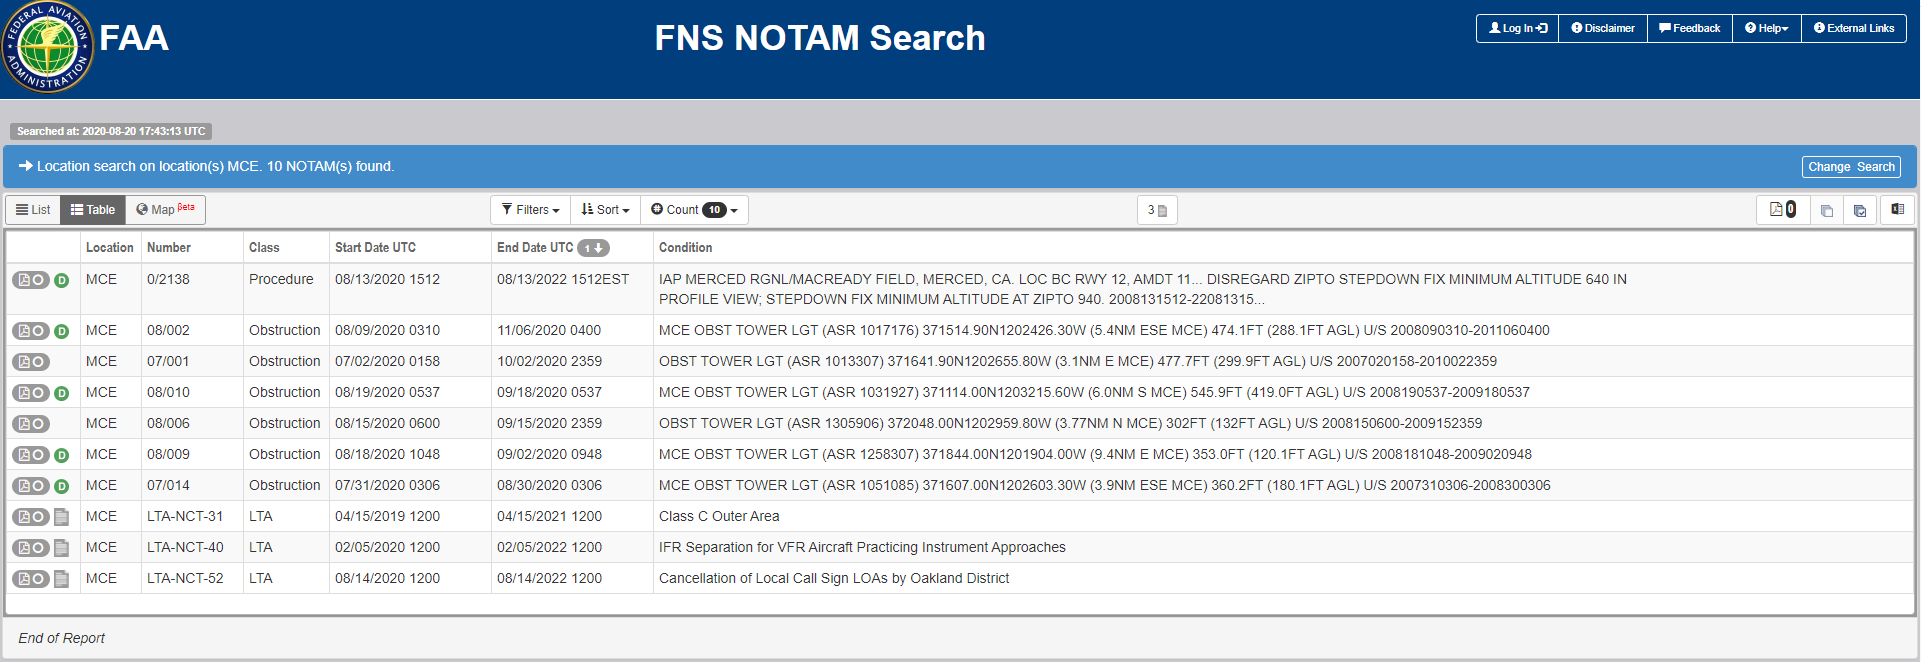
\includegraphics{images/FAA-Notam.png}
\caption{FAA NOTAM (Notice to Airman)}
\end{figure}

A NOTAM or Notice to Airman, is a notice that pertains to the establishment, change or condition of any facility, service or procedure of a specific location. The information is not known far enough in advance to be publicized by any other means therefore ensuring there are no active NOTAMS in the area you will be flying in is essential to the safety of yourself and others. It is important to keep in mind that NOTAMS can be put up at a moments notice.

\hypertarget{other-sources}{%
\section{Other Sources}\label{other-sources}}

Two other useful sources of information are \href{https://skyvector.com/}{Skyvector} and the B4UFly App (\href{https://apps.apple.com/us/app/b4ufly/id992427109}{iOS} and \href{https://play.google.com/store/apps/details?id=gov.faa.b4ufly2\&hl=en}{Android}).

\hypertarget{skyvector}{%
\subsection{SkyVector}\label{skyvector}}

\begin{figure}

{\centering 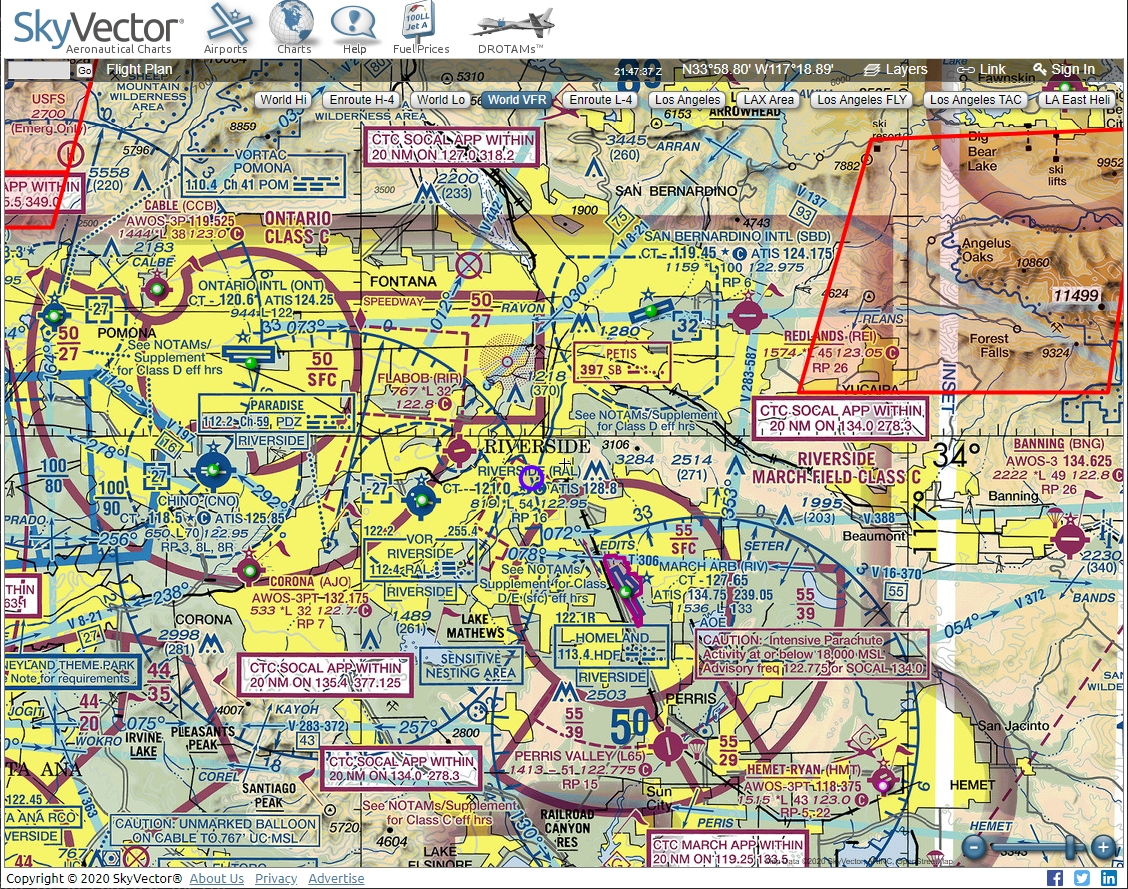
\includegraphics[width=0.9\linewidth]{images/skyvector} 

}

\caption{SkyVector - VFR Chart viewer with TFRs}\label{fig:skyvector}
\end{figure}

SkyVector is a manned aviation tool that allows users to view the FAA Sectional Charts (also known as VFR charts) as well as a wide range of other layers, including TFRs and IFR approaches. While most of the information will be overwhelming for the beginning drone pilot, the basic VFR charts are still a great resource.

\hypertarget{b4ufly-app}{%
\subsection{B4UFly App}\label{b4ufly-app}}

The B4UFly app is the FAA's first attempt at developing and publishing an app for drone pilots. It has much of the same information as Airmap, though it notably does not include the altitude limits from the UAS Facility Maps. Otherwise, it's a great source of information.

\hypertarget{airspace-regulations}{%
\section{Airspace Regulations}\label{airspace-regulations}}

On this page, we're only looking at how to get the most basic of airspace information. But obviously, there's a deeper level of knowledge to be studied when it comes to airspace regulations. You'll find more information on the UAS Regulations and Learning About Airspace page, but for now, you can take a quick look at Figure \ref{fig:SUAS-sim-regs} below.

\begin{figure}

{\centering 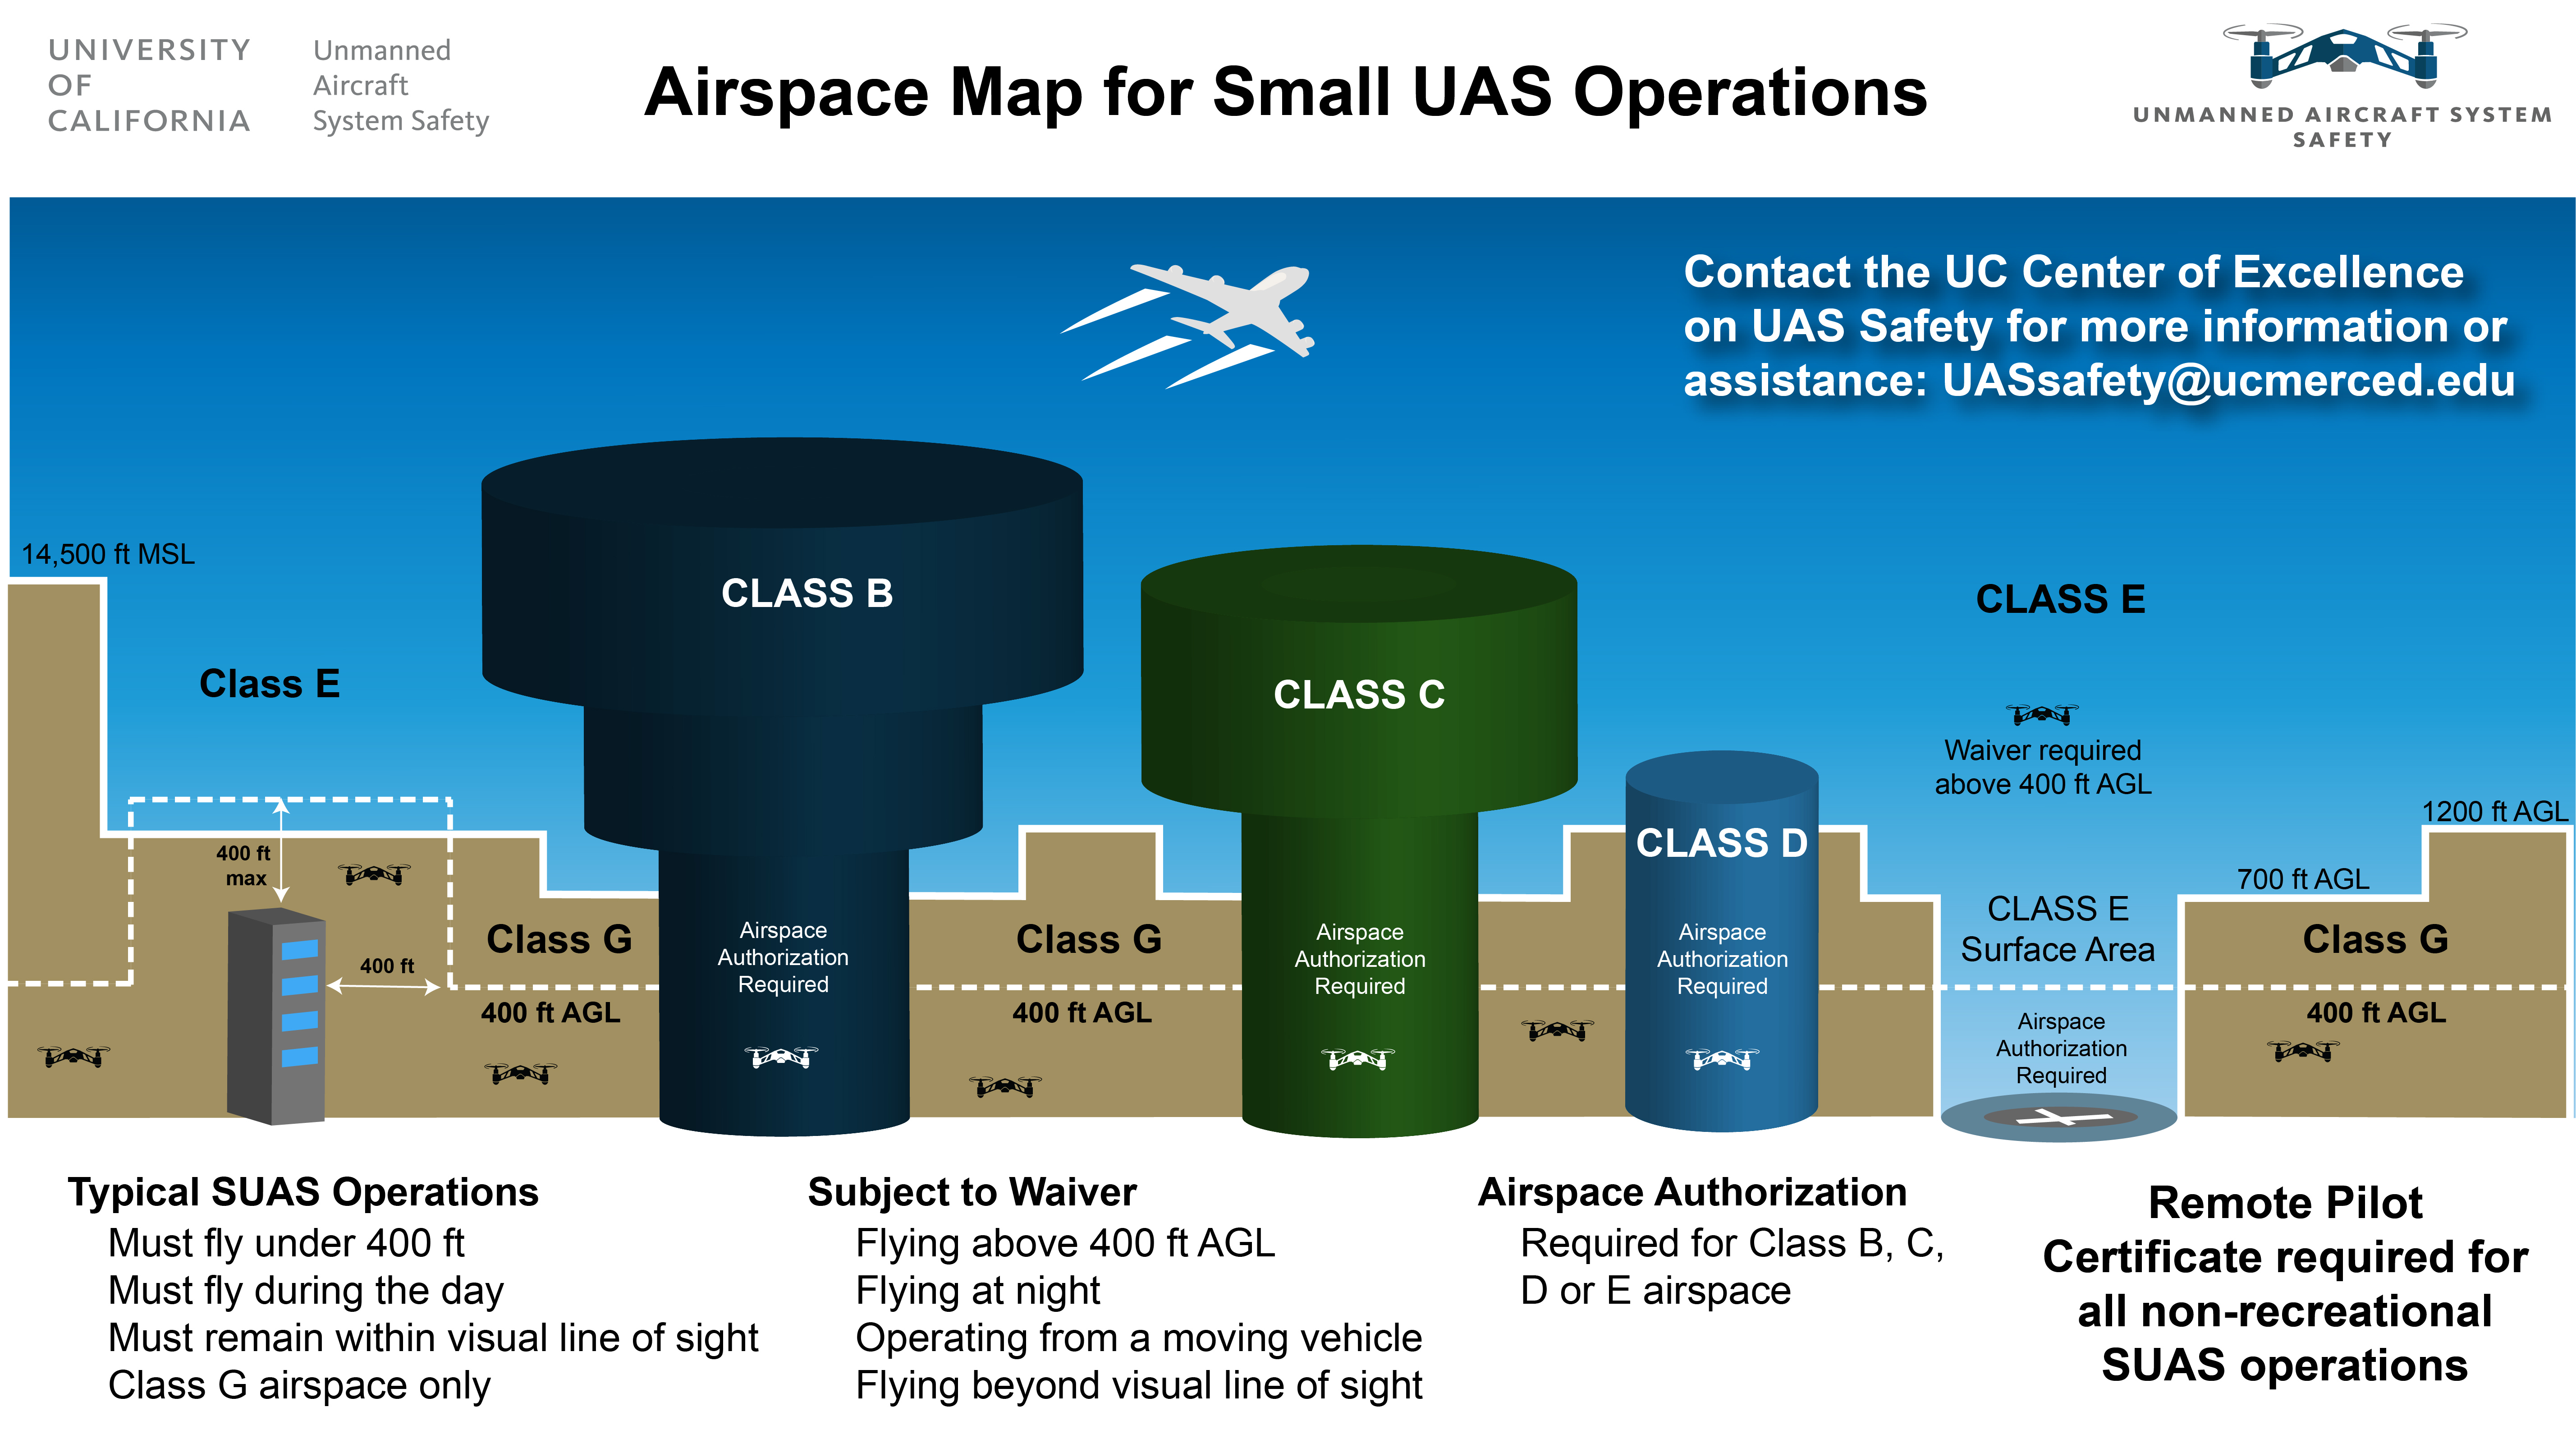
\includegraphics[width=0.9\linewidth]{images/SUAS_airspace_map} 

}

\caption{Small UAS Airspace Rules}\label{fig:SUAS-sim-regs}
\end{figure}

\hypertarget{ch-LAANC}{%
\chapter{LAANC Authorization}\label{ch-LAANC}}

In order to get FAA authorization to fly in controlled airspace, you typically will need to file a request through a system called ``LAANC''

\hypertarget{using-airmap}{%
\section{Using AirMap}\label{using-airmap}}

\hypertarget{tips-tricks}{%
\section{Tips \& Tricks}\label{tips-tricks}}

\begin{itemize}
\item
  \textbf{Need to draw a polygon using a satellite map?}

  Try this:

  \begin{itemize}
  \tightlist
  \item
    Go to \url{https://geoman.io/geojson-editor} and draw your polygon with satellite map on. Export to a GeoJSON text file
  \item
    Upload the GeoJSON file to Airmap using the `cloud' button underneath the polygon.
  \item
    The outline should now cover the right area and you file as normal
  \end{itemize}
\end{itemize}

\hypertarget{part-uc-drones}{%
\part{UC Drones}\label{part-uc-drones}}

\hypertarget{ch-about-UCdrones}{%
\chapter{About UC Drones}\label{ch-about-UCdrones}}

This is how you use UC Drones Web App

\hypertarget{part-drone-safety}{%
\part{Drone Safety}\label{part-drone-safety}}

\hypertarget{ch-safety-guidelines}{%
\chapter{Safety Guidelines}\label{ch-safety-guidelines}}

\hypertarget{ch-fire-safety}{%
\chapter{Fire Safety}\label{ch-fire-safety}}

While UAS accidents and incidents involving fire are rare, they are a valid and significant concern. With the majority of UC UAS usage on field sites and other rural locations, the potential for the accidental sparking of fire is a concern. A fire sparked by a UAS can spread quickly (Figure \ref{fig:fire-start}) and with California's dry environment, can cause significant damage (Figure \ref{fig:fire-damage}).

\begin{figure}

{\centering 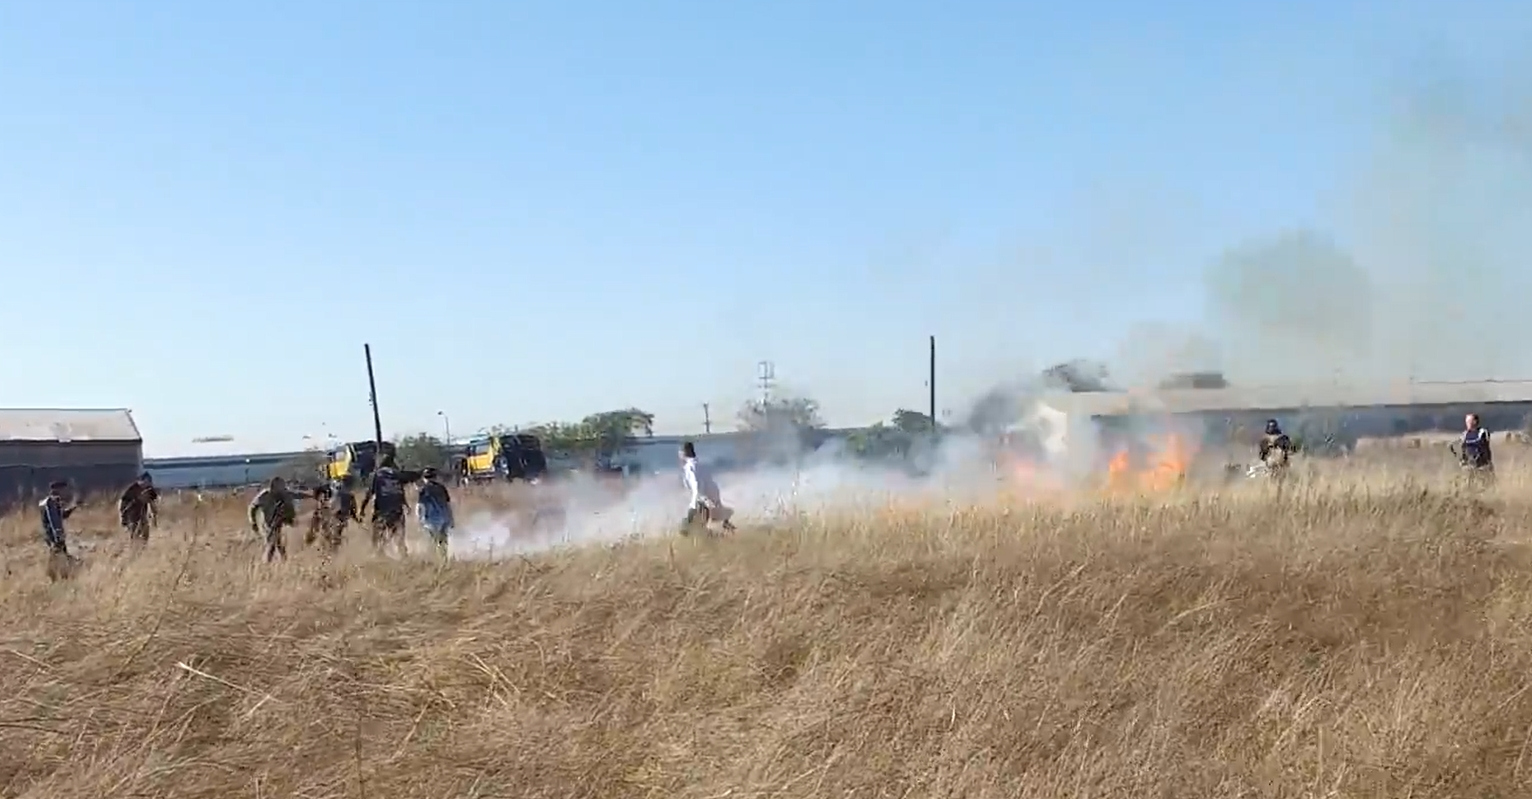
\includegraphics[width=0.75\linewidth]{images/fire_start} 

}

\caption{Beginning of a fire from UAS accident at Richmond Field Station, UC Berkeley}\label{fig:fire-start}
\end{figure}

\begin{figure}

{\centering 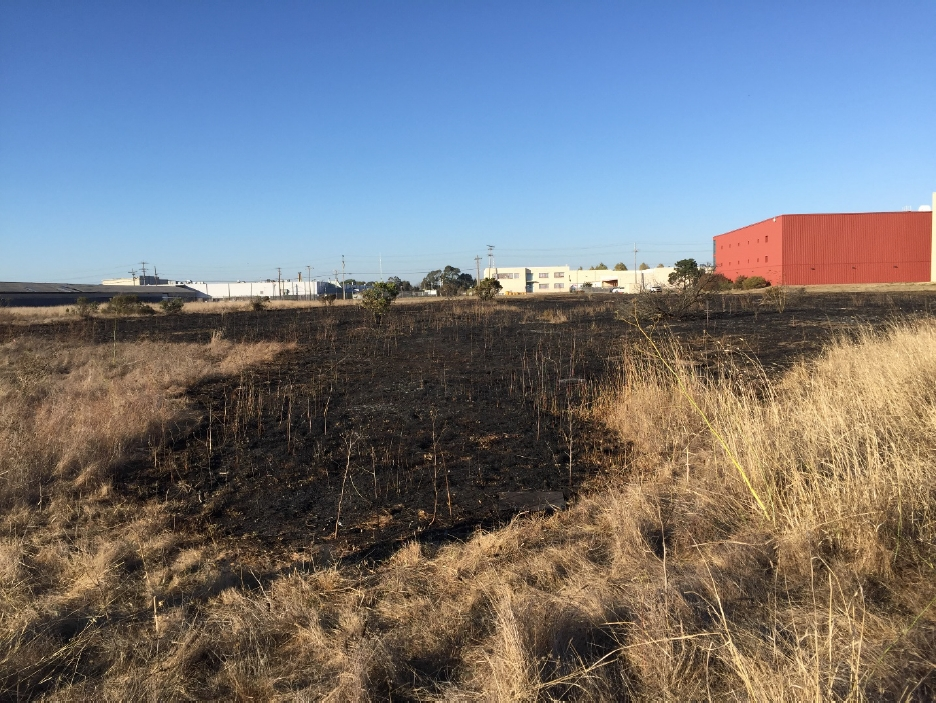
\includegraphics[width=0.75\linewidth]{images/fire_damage} 

}

\caption{Post fire damage from UAS accident at Richmond Field Station, UC Berkeley}\label{fig:fire-damage}
\end{figure}

\hypertarget{lipo-battery-guidance}{%
\section{LiPo Battery Guidance}\label{lipo-battery-guidance}}

The most common cause of UAS related fire is from misuse of LiPo batteries. Special care should be taken when charging, discharging or storing LiPo batteries. If the internal polymer cell of a LiPo battery is exposed to air, a violent chemical reaction starts that could explode, but more commonly releases significant amounts of smoke and heat that can ignite other fire fuel sources. A LiPo battery fire is typically caused by a physical puncture to the battery or from misuse, such as overcharging or electrical shorts.

\textbf{Recommended Best Practices}

\begin{itemize}
\item
  Always thoroughly inspect a battery before charging and use.

  \begin{itemize}
  \tightlist
  \item
    Look for swelling, puffy cells, cracks in plastic, and charred debris along the contacts.
  \end{itemize}
\item
  Never use a battery that is not in good health.

  \begin{itemize}
  \tightlist
  \item
    Consider batteries to be replaceable and consumable, rather than a permanent component of the UAS.
  \end{itemize}
\item
  Never store batteries in a hot car.
\item
  Don't charge your batteries unless you're going to fly within the next day.
\item
  After immediate use, place battery out of the sun but do not place within a closed container.

  \begin{itemize}
  \tightlist
  \item
    Ensure there is sufficient airflow to allow the battery to cool.
  \end{itemize}
\item
  When done flying for the day, always charge your batteries at least back up to storage level.
\item
  Do not charge an intelligent flight battery immediately after flight as the temperature may be too high. Wait until it cools down to room temperature before charging again.
\item
  Store the battery in a dry and cool place, keep out of direct sunlight and away from any liquids
\item
  Do not store or transport a battery with eyeglasses, watches, metal necklaces or other metal components that may short the battery
\item
  When in transport, store the batteries in a safe container that will protect it from damage, squeezing, puncturing or falling.
\end{itemize}

\hypertarget{planning-for-fire-mitigation}{%
\section{Planning for Fire Mitigation}\label{planning-for-fire-mitigation}}

In addition to LiPo battery care, special effort must be taken to consider the fire risks in UAS activity. Consult the appropriate department (Fire, Field Safety, EH\&S) if there are concerns over fire risk. Minimize the potential for fire by monitoring where the UAS will be flying and ensure that if a fire was to occur, the RPIC and any other persons, such as Visual Observers, are prepared to respond appropriately.

\textbf{Guidance for fire safety}

\begin{itemize}
\item
  Everyone should take a fire safety training course.
\item
  Avoid flying on high fire risk days, including \href{https://www.fire.ca.gov/programs/communications/red-flag-warnings-fire-weather-watches/}{Red Flag Warning} alerts issued by CAL FIRE.
\item
  Never fly alone in areas of moderate to high fire risk
\item
  Always bring a fire extinguisher and a shovel/bucket of sand to field sites.
\item
  During flight operations:

  \begin{itemize}
  \tightlist
  \item
    Ensure that a crew member has easy access to fire equipment.
  \item
    Ensure that a crew member has easy access to reach any location where the UA may crash.
  \item
    Ensure that a crew member has the ability to report an emergency situation and can adequately provide directions for emergency personnel to reach the site.
  \end{itemize}
\item
  When flying in high fire risk locations, use high quality, commercially available UA with enclosed electronics.
\item
  Never fly a damaged or swollen battery.
\end{itemize}

\hypertarget{part-insurance}{%
\part{Insurance}\label{part-insurance}}

\hypertarget{ch-liability-insurance}{%
\chapter{UC UAS Liability Insurance}\label{ch-liability-insurance}}

\hypertarget{ch-hull-insurance}{%
\chapter{UC UAS Replacement Insurance}\label{ch-hull-insurance}}

\hypertarget{part-more-details}{%
\part{More Details}\label{part-more-details}}

\hypertarget{ch-common-UAS-violations}{%
\chapter{Common UAS Regulation Violations}\label{ch-common-UAS-violations}}

Unless given special permission by the FAA under Part 107 regulations, you are only allowed to operate

\begin{itemize}
\tightlist
\item
  Within Visual Line of Sight
\item
  Not Over People
\end{itemize}

Unfortunately, these are two of the most common UAS violations that we see, especially with videos on the internet. Within the UC system, we are obligated to follow all applicable regulations. So even if you see someone else fly in violation of the laws, it's not ok for you to replicate it.

\hypertarget{visual-line-of-sight}{%
\section{Visual Line of Sight}\label{visual-line-of-sight}}

Visual line of sight means that the pilot of the drone must be able to see the drone throughout the entire flight in order to

\begin{itemize}
\tightlist
\item
  know the drone's location
\item
  determine the drone's attitude (orientation), altitude, and direction of flight
\item
  observe the airspace for other air traffic or hazards
\item
  determine that the drone does not endanger the life or property of another
\end{itemize}

The pilot must be \textbf{able} to do the above at all times, but doesn't have to be at all times - meaning he or she may glance at other objects, as long as the drone never leaves the pilot's ability to resume looking at the drone at any time.

At any given time, at least the pilot or any visual observers must maintain visual line of sight - meaning while the pilot is looking away, there must be a visual observer to watch the drone during that time.

\hypertarget{a-speck-in-the-sky-is-not-sufficient}{%
\subsection{A Speck in the Sky is not Sufficient}\label{a-speck-in-the-sky-is-not-sufficient}}

At all times, your drone must be close enough that you can tell which direction the drone is facing, how high it is and whether there are any hazards. If all you can see of your drone is a small dot, it means you've gone too far. In practice, your visual distance may be significantly impaired by trees or buildings in the horizon that may make it difficult to see the drone.

Common Drones and recommended max visual distance (on a clear day in a rural location)

\begin{itemize}
\tightlist
\item
  \textbf{DJI Mavic Series} 900 ft horizontal distance
\item
  \textbf{DJI Phantom Series} 1200 ft horizontal distance
\item
  \textbf{DJI Matrice 600 Pro} 3000 ft horizontal distance
\item
  \textbf{Fixed-wing (10ft wingspan)} 5000 ft horizontal distance
\end{itemize}

\hypertarget{you-must-be-able-to-assess-risk}{%
\subsection{You must be able to assess risk}\label{you-must-be-able-to-assess-risk}}

If you can't see the sky around the drone or the ground below the drone as in Figure \ref{fig:vlos}, you're not within visual line of sight.

\begin{figure}

{\centering 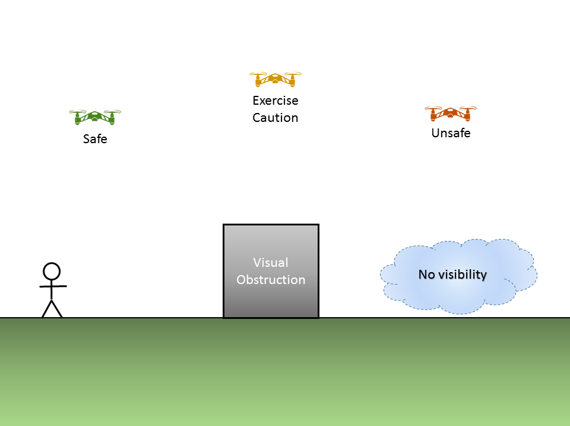
\includegraphics[width=0.8\linewidth]{images/VLOS_G} 

}

\caption{Visual Line of Sight}\label{fig:vlos}
\end{figure}

If this is a scenario that you're looking to do, you may be able to deploy a helper to assist to maintaining a clear flight operational area. However, at no point is the drone allowed to be not viewable by the pilot.

\hypertarget{operations-over-human-beings}{%
\section{Operations over Human Beings}\label{operations-over-human-beings}}

Your drone is not allowed to be flown directly over people (107.39), or in a manner that poses a hazard to other people in the event of a loss of control of the drone for any reason (107.19(c)). The combination of the two regulations form the majority of the restrictions around people.

You may only fly above people who are part of the immediate flight crew and whose tasks include ensuring flight safety. It is not sufficient to provide spectators with personal protective equipment (PPE), or ask spectators to sign waivers.

For more information about establishing effective safety buffers, see .

\hypertarget{ch-uas-accident}{%
\chapter{Reporting UAS Accidents}\label{ch-uas-accident}}

\begin{figure}
\centering
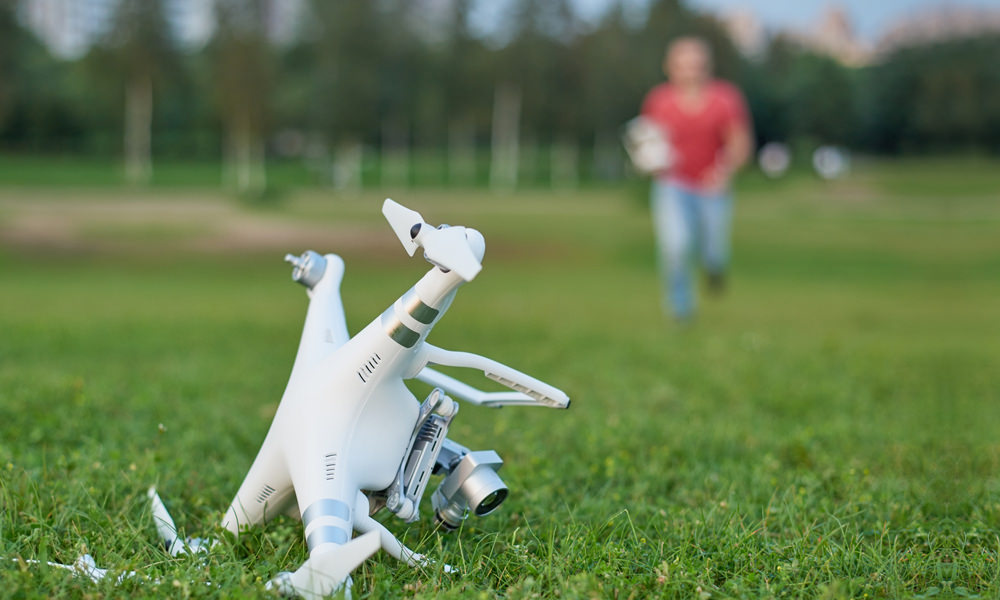
\includegraphics{images/DroneCrash.jpg}
\caption{Crashed Phantom}
\end{figure}

Whether you're a new or experienced pilot, accidents can happen. In the event that you crash your drone you need to remember to stay cool and carefully survey the damage that was caused.

If your accident causes either:

\begin{itemize}
\tightlist
\item
  Serious injury (injury that requires hospitalization) or loss of consciousness; or
\item
  More than \$500 worth of damage (excluding the drone)
\end{itemize}

then you are required to file a report with the FAA within 10 days of the accident.

\hypertarget{how-to-file-an-accident-report}{%
\section{How to file an accident report}\label{how-to-file-an-accident-report}}

You can report an accident to the FAA using a few different methods. Method 1 is to submit your report through the FAA's Drone Zone page.

\begin{figure}
\centering
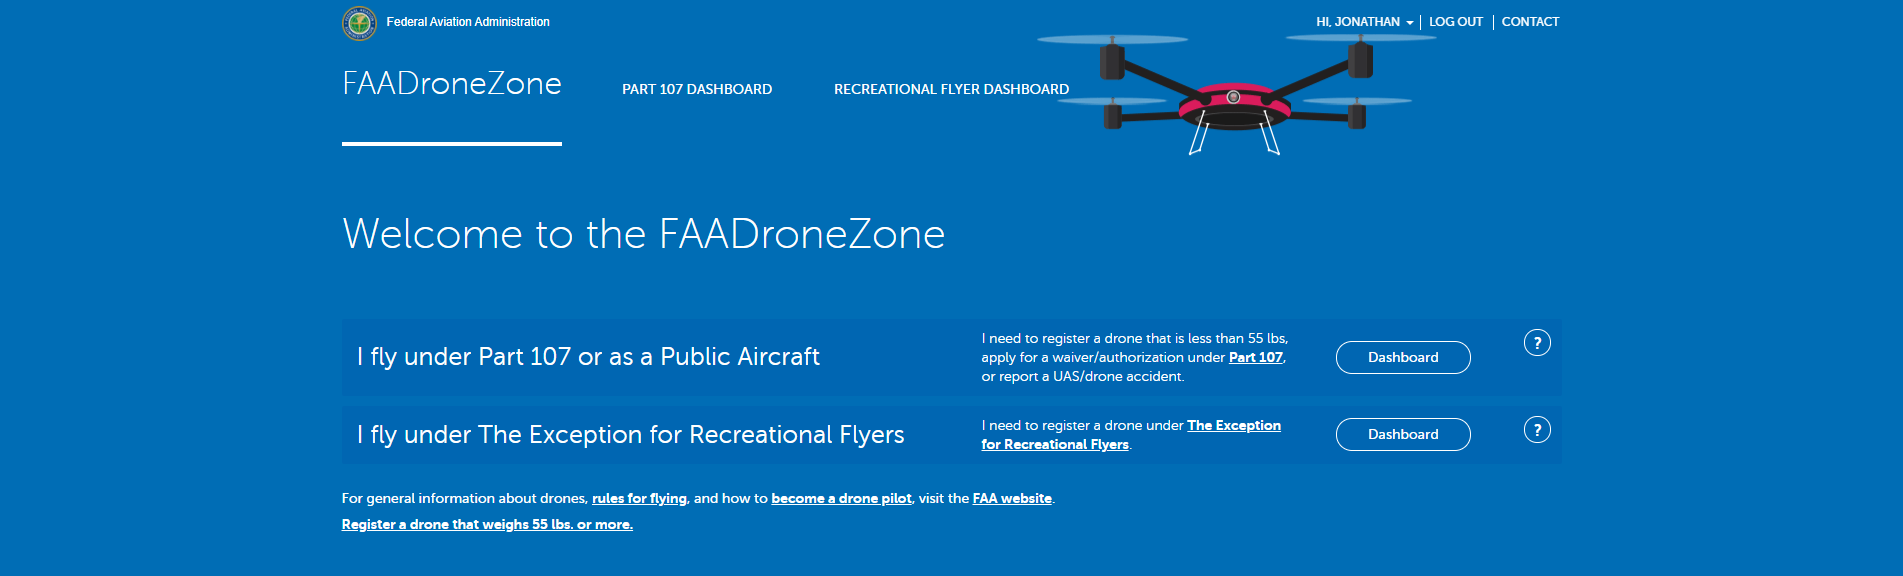
\includegraphics{images/FAA_DroneZone.png}
\caption{FAA Drone Zone}
\end{figure}

\begin{figure}
\centering
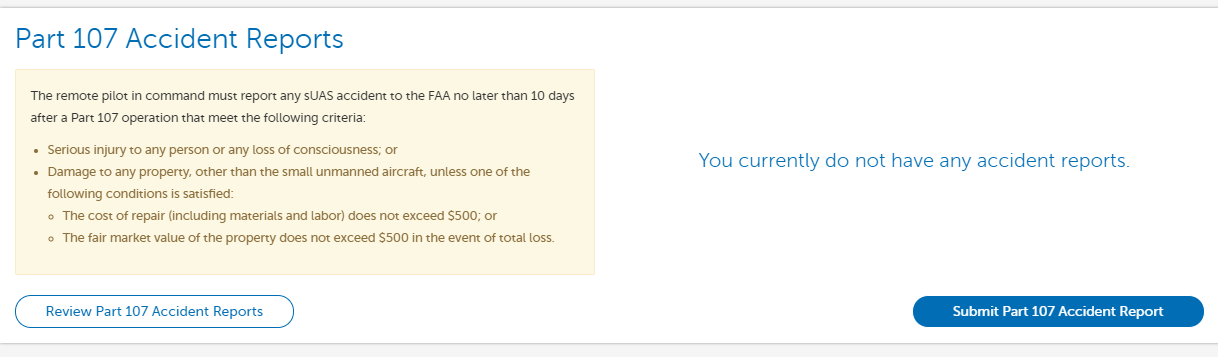
\includegraphics{images/DroneZone_AccidentReport.png}
\caption{Accident Report Box}
\end{figure}

Logging into your account and scrolling to the bottom of your dashboard you will find a ``Part 107 Accident Reports'' box where you can then submit your accident report. The reporting form requires you to fill out both plot information and your flight operation details.

\begin{figure}
\centering
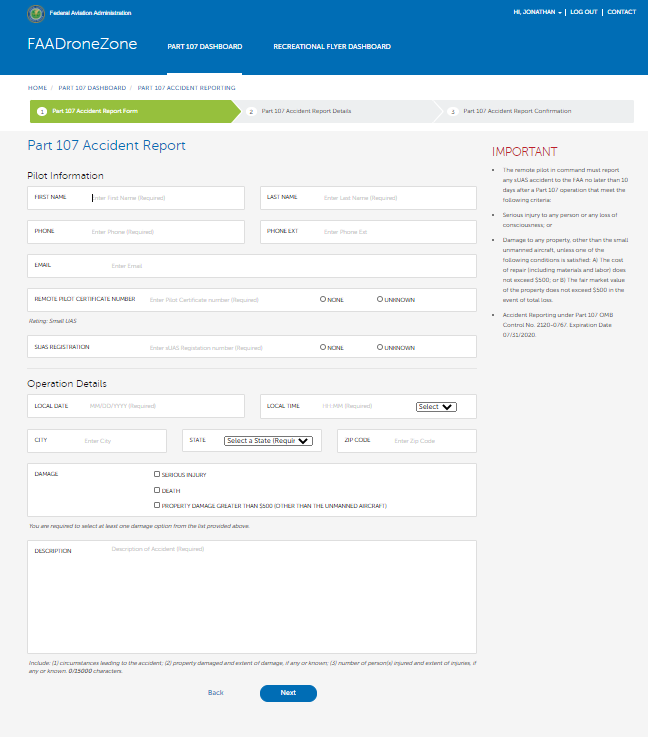
\includegraphics{images/DroneZone_Accident_Form.png}
\caption{Accident Reporting Form}
\end{figure}

Method 2 involves contacting your nearest FAA Flight Standards \href{https://www.faa.gov/about/office_org/field_offices/fsdo/}{Disctrict Office (FSDO)} to submit a report either throough phone or their website.

\begin{figure}
\centering
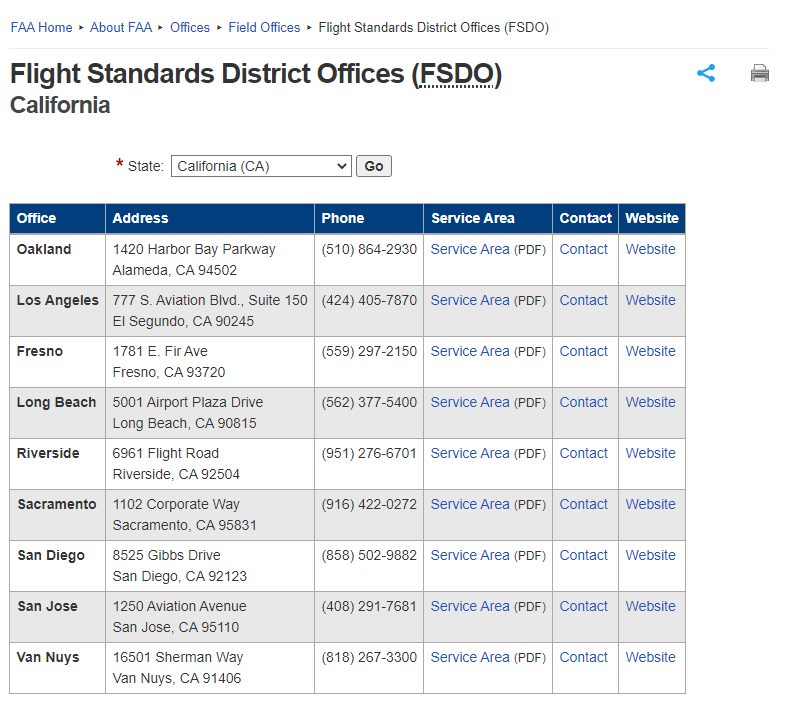
\includegraphics{images/FAA_California_FSDO.png}
\caption{Flight Standards District Offices in California}
\end{figure}

\hypertarget{ch-local-UAS-regulations}{%
\chapter{Local UAS Regulations}\label{ch-local-UAS-regulations}}

Any regulatory agency or private property owner can make rules and regulations within their jurisdiction (within reason). The FAA's jurisdiction is the sky and aviation support (licensing, registration, infrastructure).

However, there are other aspects of UAS activity that may be subject to local rules and regulations.

State and local powers include

\begin{itemize}
\tightlist
\item
  Land Use
\item
  Trespass
\item
  Privacy
\item
  Noise ordinances
\item
  Wildlife conservation
\item
  Insurance
\end{itemize}

It is allowed for a State, county or city to place restrictions on where and when drones may take off and land (land use jurisdiction), to define what constitutes invasion of privacy, or to require insurance to operate for or within a jurisdiction. It is your responsibility to

The UC Center of Excellence will help assist you in identifying applicable local regulations, however you are responsible for ensuring your regulatory compliance with all local regulations.

\hypertarget{searching-for-local-uas-regulations}{%
\section{Searching for Local UAS Regulations}\label{searching-for-local-uas-regulations}}

There is no easy database for applicable UAS regulations - you will likely have to search multiple locations. Most county and state owned land that is set aside for conservation often have established processes for research permits that are good starting points for UAS use.

Some good resources:

\begin{itemize}
\tightlist
\item
  State level regulations are typically associated with state managed lands, wildlife conservation, privacy and insurance.
\item
  County and Municipal Codes often include regulations for city/county parks and open spaces, typically on land use, trespass and privacy.
\item
  Directors or on-site managers are often good people to ask for permit processes and costs
\end{itemize}

\hypertarget{no-drone-zones}{%
\section{No Drone Zones}\label{no-drone-zones}}

Please respect local ordinances, even if you do not agree with them. Do not look for ways to circumvent or utilize a loophole if it is counter to the local communities desires. If you are operating for research or education, you are acting as a representative of the University of California, and we strive to be good neighbors and collaborative with all communities.

\begin{figure}

{\centering 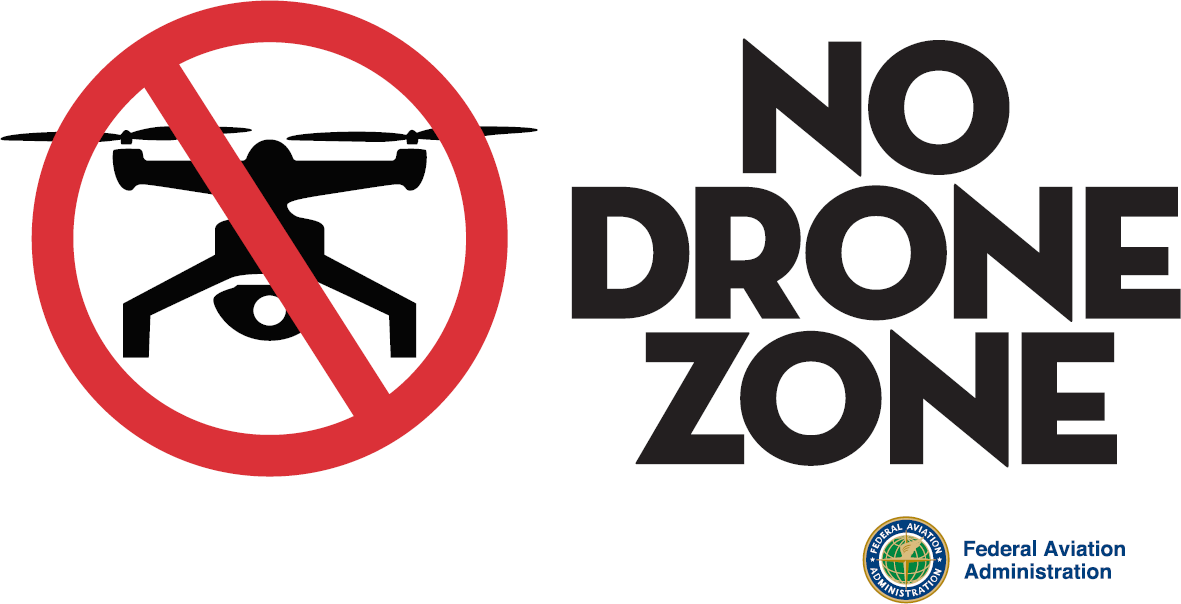
\includegraphics[width=0.8\linewidth]{images/no-drone-zone} 

}

\caption{No Drone Zone Sign}\label{fig:no-drone-zone}
\end{figure}

If you feel strongly, engage the local community in outreach and discussion and work to change their views. But recognize that what you want may not ever be what they want, and you may not be able to change their minds. If you are struggling to get access to your desired site, feel free to reach out to us and we'll see if we can find an alternative location.

\hypertarget{ch-replace-license}{%
\chapter{Update or Replace a License}\label{ch-replace-license}}

Did you move or change names? Remember that you must inform the FAA within 30 days.

The easiest way to update your information with the FAA is through the Airmen Services page: \url{https://amsrvs.registry.faa.gov/amsrvs/default.asp} (Figure \ref{fig:airmen-services})

On this page, you can

\begin{itemize}
\tightlist
\item
  Change your address
\item
  Order a replacement certificate (\$2)
\item
  Change status of address releasability (by default, all addresses on pilot licenses, including drone licenses are public)
\item
  Remove SSN as certificate number (for those with older manned aviation licenses)
\item
  Request verification of certificate privileges
\end{itemize}

\begin{figure}

{\centering 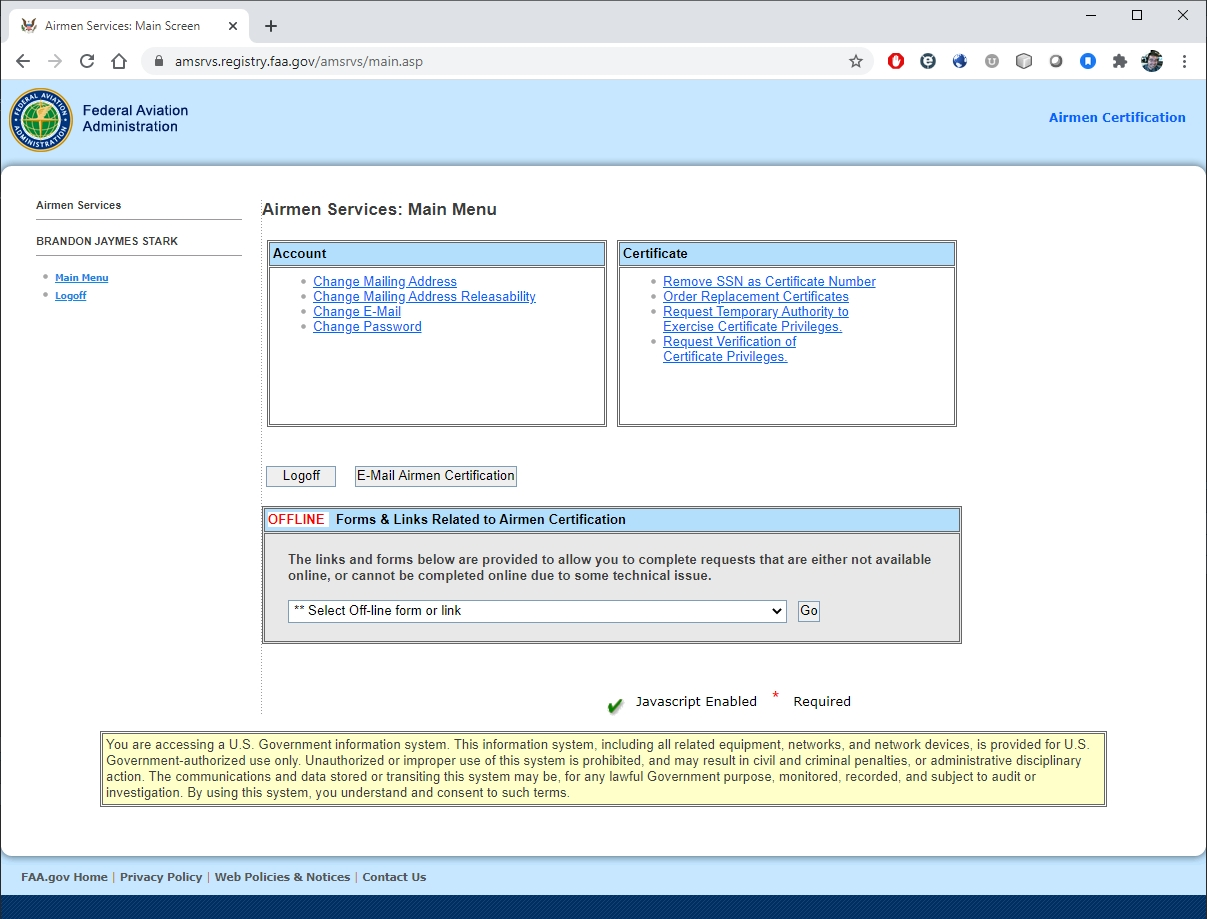
\includegraphics[width=0.7\linewidth]{images/airmen-services} 

}

\caption{FAA Airmen Services Web Page}\label{fig:airmen-services}
\end{figure}

You do not need to order a new Remote Pilot Certificate when you update your address, but ordering a replacement certificate is the only way that you'll get a new copy of your certificate with your new address.

\end{document}
